%%%%%%%%%%%%%%%%%%%%%%%%%%%%%%%%%%%%%%%%%%%%%%%%%%%%%%
% A Beamer template for University of Wollongong     %
% Based on THU beamer theme                          %
% Author: Qiuyu Lu                                   %
% Date: July 2024                                    %
% LPPL Licensed.                                     %
%%%%%%%%%%%%%%%%%%%%%%%%%%%%%%%%%%%%%%%%%%%%%%%%%%%%%%
% Customized for Sharif University of Technology     %
%%%%%%%%%%%%%%%%%%%%%%%%%%%%%%%%%%%%%%%%%%%%%%%%%%%%%%


\documentclass[serif, aspectratio=169]{beamer}
%\documentclass[serif]{beamer}  % for 4:3 ratio
\usepackage[T1]{fontenc} 
\usepackage{fourier} % see "http://faq.ktug.org/wiki/uploads/MathFonts.pdf" for other options
\usepackage{hyperref}
\usepackage{latexsym,amsmath,xcolor,multicol,booktabs,calligra}
\usepackage{graphicx,pstricks,listings,stackengine}
\usepackage{lipsum}
\usepackage{array}
\usepackage{tikz}
\usepackage{tcolorbox}
\usepackage{graphicx}
\usepackage{amsfonts}
\usepackage{hyperref}


\usetikzlibrary{positioning,calc}





\author{Ali Sharifi-Zarchi}
\title{Machine Learning (CE 40717)}
\subtitle{Fall 2024}
\institute{
    CE Department \\
    Sharif University of Technology
}
%\date{\small \today}
% \usepackage{UoWstyle}
\usepackage{SUTstyle}

% defs
\def\cmd#1{\texttt{\color{red}\footnotesize $\backslash$#1}}
\def\env#1{\texttt{\color{blue}\footnotesize #1}}
\definecolor{deepblue}{rgb}{0,0,0.5}
\definecolor{deepred}{RGB}{153,0,0}
\definecolor{deepgreen}{rgb}{0,0.5,0}
\definecolor{halfgray}{gray}{0.55}


% Define custom colors
\definecolor{blue!20}{RGB}{173, 216, 230}
\definecolor{green!20}{RGB}{144, 238, 144}
\definecolor{red!20}{RGB}{255, 182, 193}

\lstset{
    basicstyle=\ttfamily\small,
    keywordstyle=\bfseries\color{deepblue},
    emphstyle=\ttfamily\color{deepred},    % Custom highlighting style
    stringstyle=\color{deepgreen},
    numbers=left,
    numberstyle=\small\color{halfgray},
    rulesepcolor=\color{red!20!green!20!blue!20},
    frame=shadowbox,
}


\begin{document}

\begin{frame}
    \titlepage
    \vspace*{-0.6cm}
    \begin{figure}[htpb]
        \begin{center}
            
\includegraphics[keepaspectratio, scale=0.25]{pic/sharif-main-logo.png}
        \end{center}
    \end{figure}
\end{frame}

\begin{frame}    
\tableofcontents[sectionstyle=show,
subsectionstyle=show/shaded/hide,
subsubsectionstyle=show/shaded/hide]
\end{frame}



\section{Task Introduction}

\begin{frame}{Problem Setup}
    \vspace{-0.1cm}

    \begin{columns}[t] % Use top alignment for better layout control
        % Left column with "Before..."
        \begin{column}{0.5\textwidth}
            \textbf{Before...} % Remove center alignment for left-alignment
            \vspace{0.2cm}
            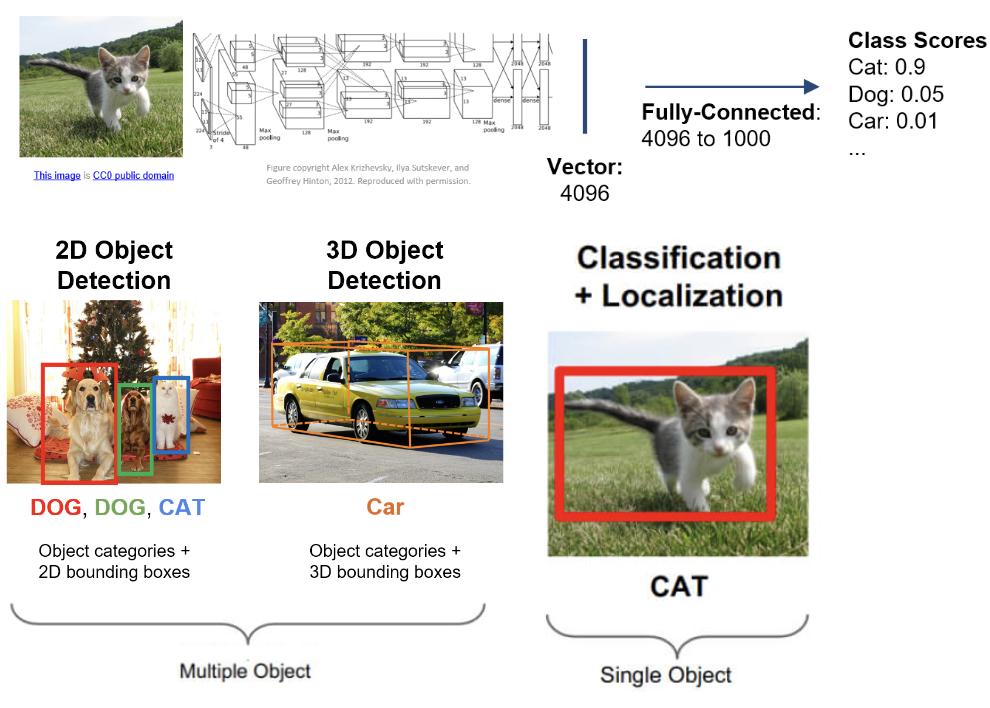
\includegraphics[width=\textwidth]{pic/SS problem setup before.png}
        \end{column}
        
        \begin{column}{0.5\textwidth}
            \textbf{Now...}
            \vspace{0.2cm}
            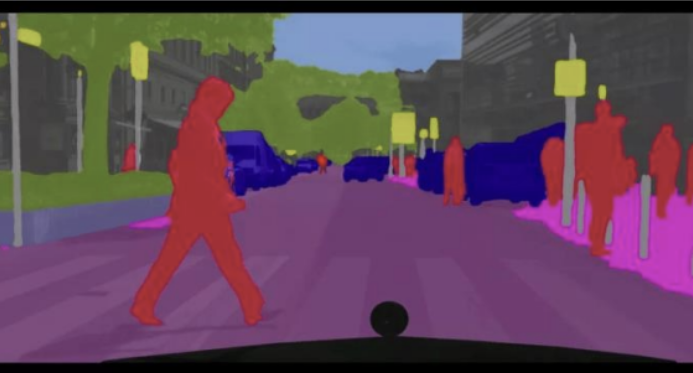
\includegraphics[width=\textwidth]{pic/SS problem setup now1.png} 
        \end{column}
    \end{columns}
    
     \textbf{\textcolor{deepred}{Problem:}} \textcolor{deepred}{We want the output to have the same resolution as the input!}
    % Text below the "Now..." section
    \begin{itemize}
        \item Label every single pixel with its class. Actually simpler in some sense:
        \begin{itemize}
            \item[] \textbullet \ No longer variable \# of outputs. \hspace{1em}\textbullet \ Every pixel has a label.
        \end{itemize}
    \end{itemize}

\end{frame}


\begin{frame}{Problem Setup}
    \begin{center}
        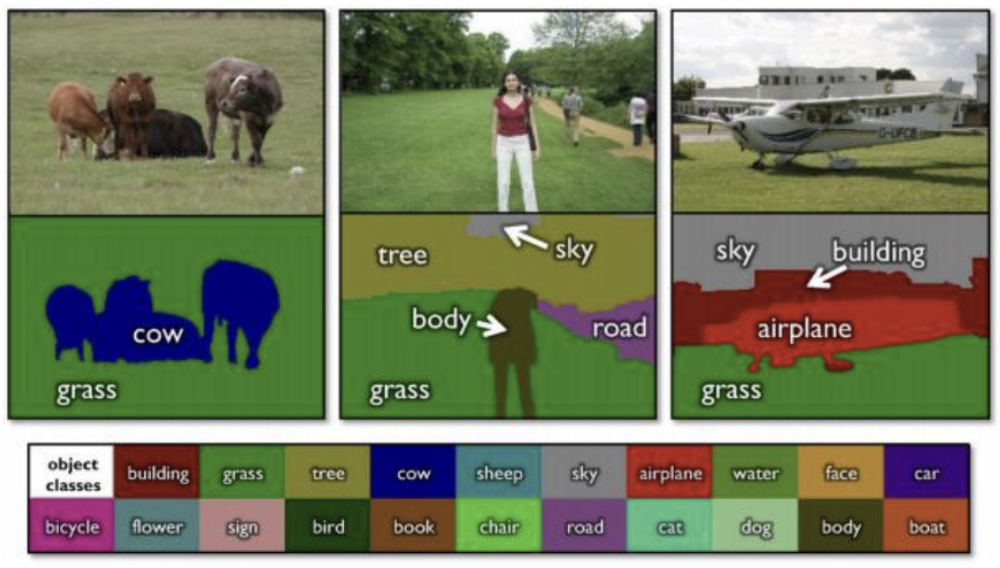
\includegraphics[width=0.5\textwidth]{pic/SS problem setup now2.png}
    \end{center}
    
    
    \begin{minipage}{0.9\textwidth}\footnotesize
        \textbf{Classify every point with a class} \\
        Don't worry for now about instances (e.g., two adjacent cows are just one "cow blob" and that’s OK for some reason)\\

                
        \textbf{The challenge: design a network architecture} \\
        that makes this \textbf{"per-pixel classification"} problem  \color{deepblue}{computationally tractable}
    \end{minipage}
\end{frame}


\begin{frame}{Semantic Segmentation: Sliding Window}
    \begin{center}
        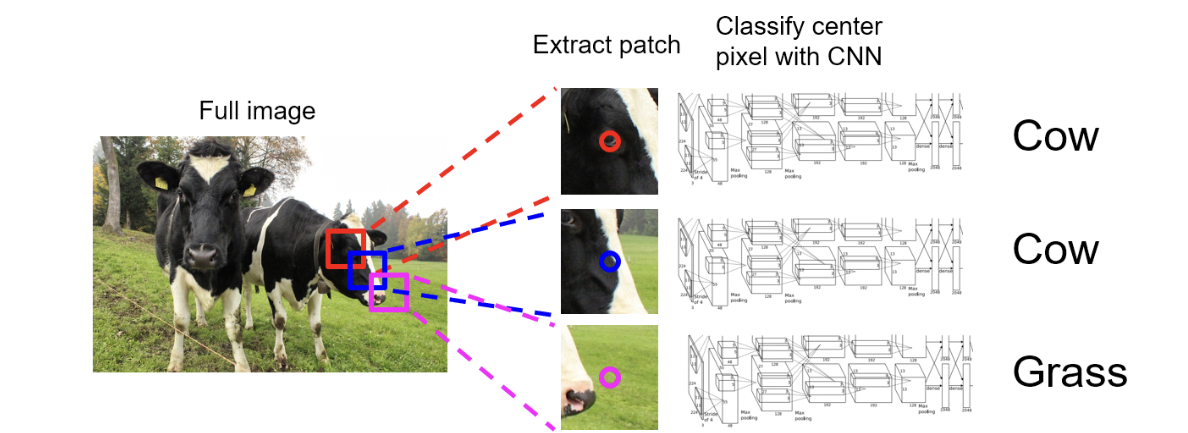
\includegraphics[width=0.9\textwidth]{pic/SS sliding window.png}
    \end{center}
    
    \vspace{0.3cm}
    
    \textcolor{deepred}{\textbf{Problem: Very inefficient! Not reusing shared features between overlapping patches}}
    
    \vspace{0.3cm}
    
    \scriptsize{
    Farabet et al., “Learning Hierarchical Features for Scene Labeling,” TPAMI 2013 \\
    Pinheiro and Collobert, “Recurrent Convolutional Neural Networks for Scene Labeling,” ICML 2014
    }
    \vspace{0.2cm}

\end{frame}

\begin{frame}{Semantic Segmentation Idea: Fully Convolutional}
  
    
    \begin{center}
        Design a network as a bunch of convolutional layers \\
        to make predictions for pixels all at once!
    \end{center}

      \begin{center}
        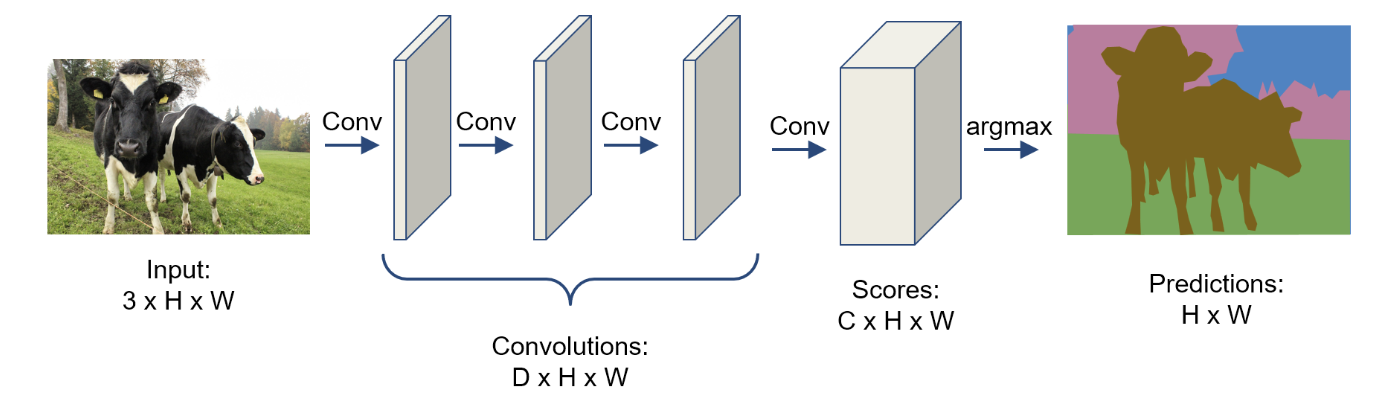
\includegraphics[width=0.9\textwidth]{pic/SS fully conv1.png}
    \end{center}
    
    \vspace{0.1cm}
    
    
    \textcolor{deepred}{\textbf{Problem: convolutions at original image resolution will be very expensive ...}}
\end{frame}

\begin{frame}{Semantic Segmentation Idea: Fully Convolutional}
    \textcolor{deepgreen}{\textbf{So far we learn about downsampling...}}

    \begin{center}
        \vspace{0.3cm}
        Design network as a bunch of convolutional layers, \\
        with \textcolor{red}{downsampling} and \textcolor{blue}{upsampling} inside the network!
    \end{center}
    
    \begin{center}
        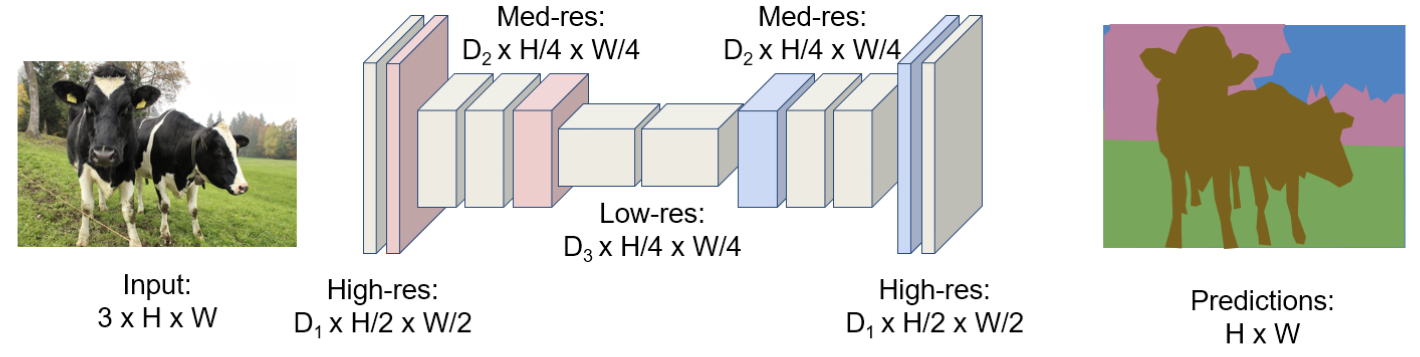
\includegraphics[width=0.9\textwidth]{pic/SS fully conv2.png}
    \end{center}
    
    \vspace{0.5cm}
    
    \scriptsize{
    Long, Shelhamer, and Darrell, “Fully Convolutional Networks for Semantic Segmentation,” CVPR 2015 \\
    Noh et al., “Learning Deconvolution Network for Semantic Segmentation,” ICCV 2015
    }
\end{frame}

\begin{frame}{Recap: Types of Downsampling}
    \begin{itemize}
        \item Max Pooling
        \item Average Pooling
        \item Global Average Pooling
        \item Strided Convolution
        \item Spatial Pyramid Pooling
        \item \ldots
    \end{itemize}
\end{frame}

\begin{frame}{Details of Downsampling Methods}
    \scriptsize
    \begin{table}[]
        \centering
        \renewcommand{\arraystretch}{1.2} % Slightly increase row height for readability
        \begin{tabular}{|p{2.5cm}|p{3.5cm}|p{2.8cm}|p{3.5cm}|}
            \hline
            \textbf{Pooling Method} & \textbf{Key Features} & \textbf{Best Applications} & \textbf{Rule of Thumb} \\ \hline
            Max Pooling & Captures the most important feature in a region (e.g., edges) & Image classification, object detection & Use when sharp features (e.g., edges) are essential. \\ \hline
            Average Pooling & Smooths the feature map, averages over a region & Smoothing features, object detection & Use for smoother output, where fine detail is less important. \\ \hline
            Global Average Pooling (GAP) & Replaces fully connected layers, outputs a single value per channel & Final layer in classification networks (e.g., ResNet, Inception) & Ideal for reducing model complexity and overfitting. \\ \hline
            Strided Convolution & Combines downsampling and feature extraction & Object detection, fully convolutional networks (FCNs) & Use for efficiency when feature extraction and downsampling can be combined. \\ \hline
            Spatial Pyramid Pooling (SPP) & Captures multi-scale features with pooling at multiple scales & Multi-scale object detection, semantic segmentation & Use when recognizing objects at various scales is critical. \\ \hline
        \end{tabular}
    \end{table}
\end{frame}

\begin{frame}{Fully Convolutional Networks (FCN)}
 
    \begin{center}
      Design network as a bunch of convolutional layers,
        \\ with \textcolor{red}{downsampling} and \textcolor{blue}{upsampling} inside the network!
        \vspace{0.2cm}

        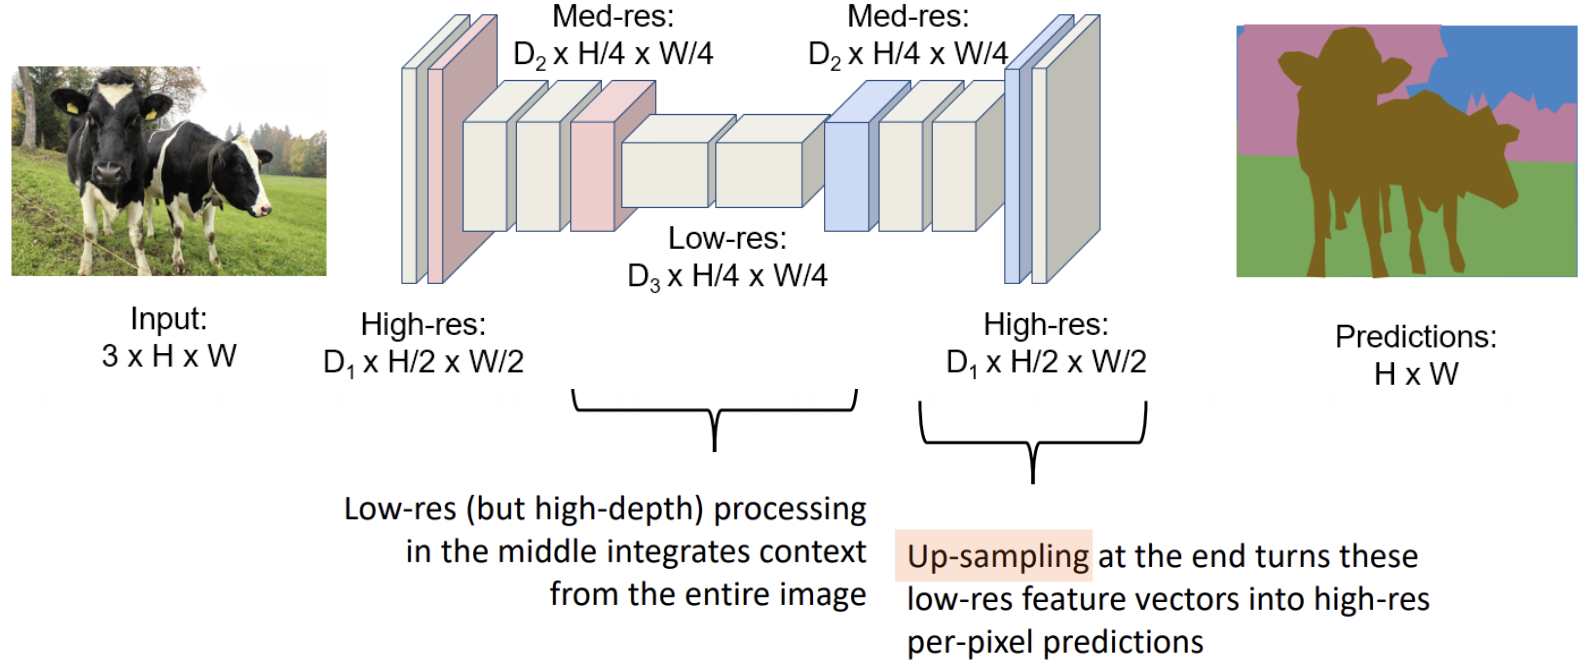
\includegraphics[width=0.9\textwidth]{pic/SS fully conv3.png}
    \end{center}

\end{frame}


\section{Transposed Convolution}

\begin{frame}{Up Samplings}
    \begin{itemize}
        \item[] We can divide methods into:
        \vspace{0.3cm}
        \item Static up sampling's
        \item Learnable up sampling's
    \end{itemize}
\end{frame}


\begin{frame}{Static Upsampling: ``Unpooling''}

\begin{columns}[c]
    % Left Column
    \begin{column}{0.5\textwidth}
        \centering
        \textbf{"Nearest Neighbor"}\\
        \vspace{0.3cm}
        \begin{tabular}{|c|c|}
            \hline
            1 & 2 \\ \hline
            3 & 4 \\ \hline
        \end{tabular}
        \hspace{0.3cm} $\longrightarrow$ \hspace{0.3cm}
        \begin{tabular}{|c|c|c|c|}
            \hline
            1 & 1 & 2 & 2 \\ \hline
            1 & 1 & 2 & 2 \\ \hline
            3 & 3 & 4 & 4 \\ \hline
            3 & 3 & 4 & 4 \\ \hline
        \end{tabular}
        \vspace{0.3cm}\\
          \begin{flushleft}
        \text{ \hspace{0.4cm} Input: 2 x 2 \hspace{1.2cm} Output: 4 x 4}
        \end{flushleft}
    \end{column}

    % Right Column
    \begin{column}{0.5\textwidth}
        \centering
        \textbf{``Bed of Nails''}\\
        \vspace{0.3cm}
        \begin{tabular}{|c|c|}
            \hline
            1 & 2 \\ \hline
            3 & 4 \\ \hline
        \end{tabular}
        \hspace{0.3cm} $\longrightarrow$ \hspace{0.3cm}
        \begin{tabular}{|c|c|c|c|}
            \hline
            1 & 0 & 2 & 0 \\ \hline
            0 & 0 & 0 & 0 \\ \hline
            3 & 0 & 4 & 0 \\ \hline
            0 & 0 & 0 & 0 \\ \hline
        \end{tabular}
        \vspace{0.3cm}\\
        \begin{flushleft}
        \text{ \hspace{0.4cm} Input: 2 x 2 \hspace{1.2cm} Output: 4 x 4}
        \end{flushleft}
    \end{column}
\end{columns}

\end{frame}



\begin{frame}{Static Upsampling: ``Max Unpooling''}
 
    \begin{center}
        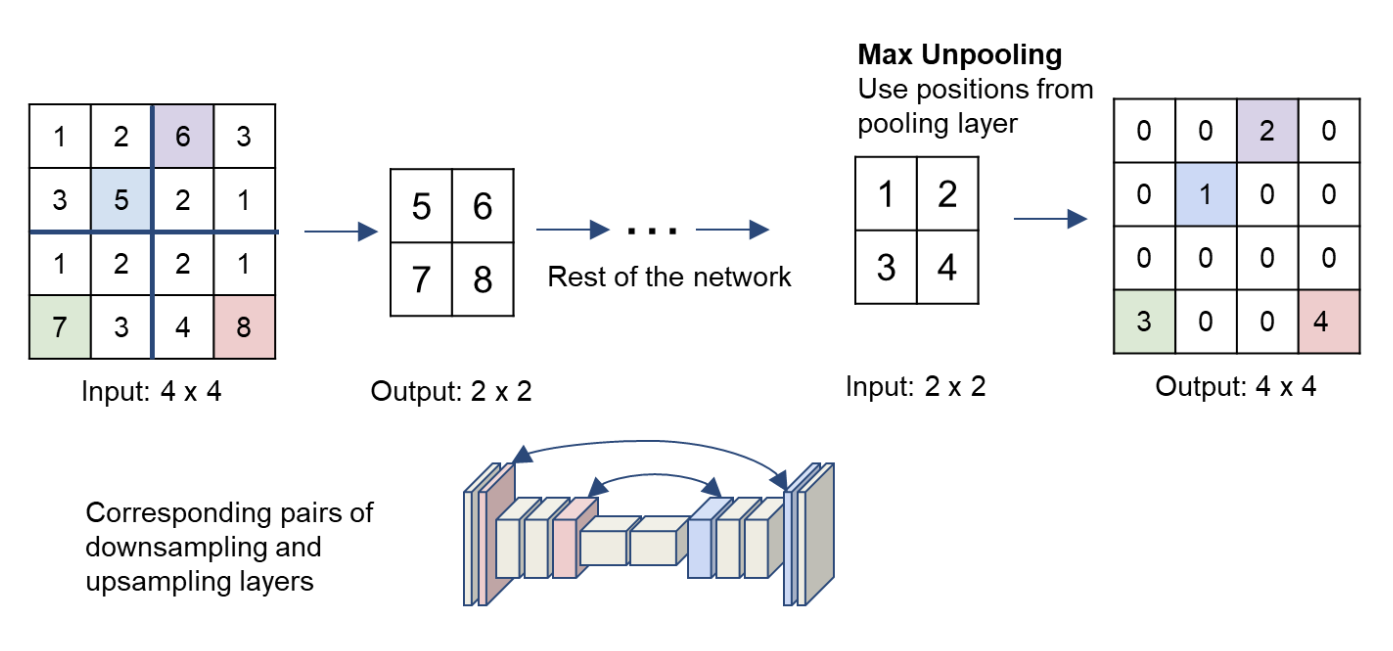
\includegraphics[width=\textwidth]{pic/Max Unpooling.png}
    \end{center}

\end{frame}


\begin{frame}{Static Upsamplings}
 
    \begin{center}
        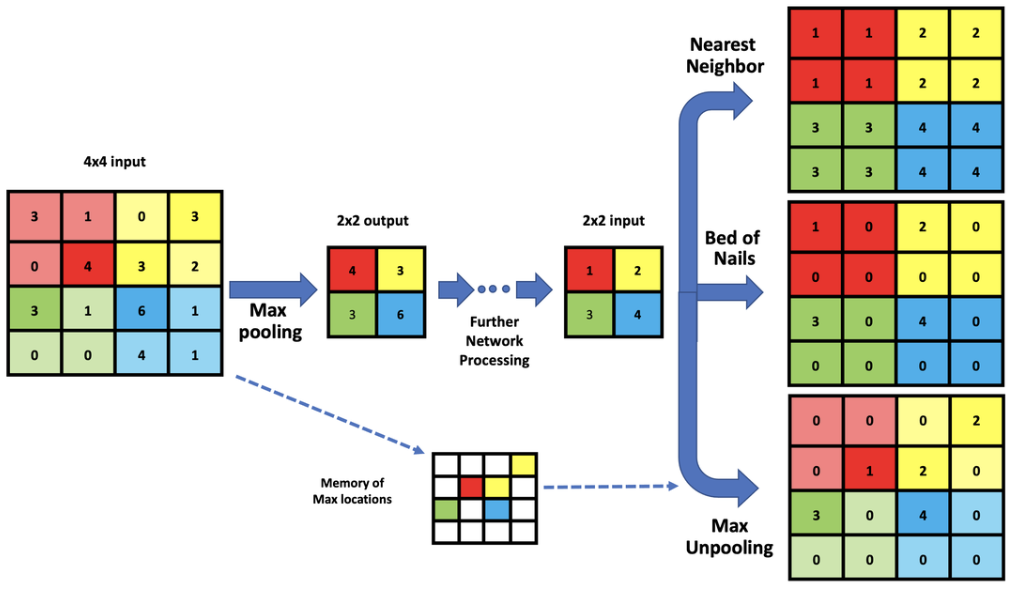
\includegraphics[width=0.75\textwidth]{pic/Static Upsampling.png}
    \end{center}
        \tiny{Image from \href{https://mriquestions.com/upsampling.html}{this link}}


\end{frame}

\begin{frame}{Convolution and Transposed Convolution}
\small
\vspace{-0.3cm}

% Main content in two columns
\begin{columns}[T]

    % Left Column for Normal Convolution
    \begin{column}{0.5\textwidth}
        \textbf{Normal Convolutions:} reduce resolution with \textbf{stride}\\
        \begin{center}
            \textbf{Stride = 2}\\
            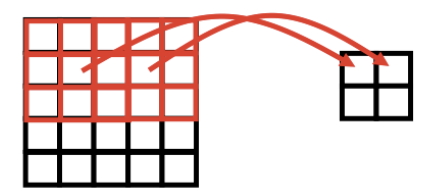
\includegraphics[width=0.8\textwidth]{pic/Conv vs Transpose Conv1.png}\\ 
            \vspace{0.75cm}
            \textbf{Input:} \( H_f \times W_f \times C_{in} \) \\
            \textbf{Output:} \( 1 \times 1 \times C_{out} \) \\
            \textbf{Filter:} \( H_f \times W_f \times C_{in} \times C_{out} \)
        \end{center}
    \end{column}

    % Right Column for Transposed Convolution
    \begin{column}{0.5\textwidth}
        \textbf{Transposed Convolutions:} increase resolution with \textbf{fractional ``stride''}\\
        \begin{center}
            \textbf{Stride = 1/2}\\
            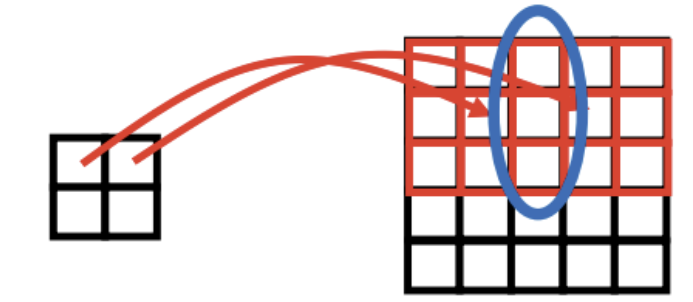
\includegraphics[width=0.85\textwidth]{pic/Conv vs Transpose Conv2.png}\\ 
              \textcolor{deepblue}{We have two sets of values here,} \textbf{\textcolor{deepblue}{sum up them!}}\\
            \vspace{0.2cm}
            \textbf{Input:} \( 1 \times 1 \times C_{in} \) \\
            \textbf{Output:} \( H_f \times W_f \times C_{out} \) \\
            \textbf{Filter:} \( C_{in} \times H_f \times W_f \times C_{out} \)
        \end{center}
    \end{column}

\end{columns}

\end{frame}


\begin{frame}{1D Convolution: A Matrix Perspective}
\small
\begin{itemize}
    \item Display the convolution matrix with a 1D kernel \([1, 1, 1]\) sliding over an input vector.
\end{itemize}

\vspace{0.3cm}

\[
\begin{bmatrix}
    1 & 1 & 1 & 0 & \dots & 0 \\
    0 & 1 & 1 & 1 & \dots & 0 \\
    0 & 0 & 1 & 1 & 1 & 0 \\
    \vdots & \vdots & \vdots & \ddots & \vdots & \vdots \\
    0 & \dots & 0 & 1 & 1 & 1
\end{bmatrix}
\begin{bmatrix}
    x_1 \\
    x_2 \\
    x_3 \\
    \vdots \\
    x_n
\end{bmatrix}
\]

\vspace{0.5cm}

\begin{itemize}
    \item This representation mimics a sliding window operation where the kernel moves across the input, performing element-wise multiplications and summing up the results.
\end{itemize}

\end{frame}


\begin{frame}{1D Transposed Convolution: A Matrix Perspective}
\small
\begin{itemize}
    \item The operation is equivalent to taking the transpose of the kernel matrix and applying it to the input:
\end{itemize}

\[
\begin{bmatrix}
    1 & 0 & 0 & 0 & \cdots & 0 \\
    1 & 1 & 0 & 0 & \cdots & 0 \\
    1 & 1 & 1 & 0 & \cdots & 0 \\
    \cdots & 1 & 1 & 1 & 0 & 0 \\
    \cdots & \cdots & 1 & 1 & 1 & 0 \\
    \cdots & \cdots & \cdots & 1 & 1 & 1 \\
    0 & 0 & 0 & \cdots & 1 & 1
\end{bmatrix}
\begin{bmatrix}
    x_1 \\ x_2 \\ x_3 \\ \vdots \\ x_k
\end{bmatrix}
\quad = \quad
\begin{bmatrix}
    A_1 & A_2 & \cdots & A_k
\end{bmatrix}
\begin{bmatrix}
    x_1 \\ x_2 \\ \vdots \\ x_k
\end{bmatrix}
= \sum_{i=1}^k x_i A_i
\]


\begin{columns}[T]
    \begin{column}{0.75\textwidth}
      \vspace{0.3cm}
        \begin{itemize}
            \item Since the transposed convolution uses the \textbf{transpose} of the kernel matrix and effectively reverses the compression process (convolution), it’s called \textbf{"Transposed Convolution"}.
        \end{itemize}
    \end{column}

  \begin{column}{0.34\textwidth}
    \scriptsize
    \textbf{Other names:}
    \vspace{-0.2cm}
    \begin{itemize}
        \setlength{\itemsep}{0pt} % Adjust the space between items
        \setlength{\parskip}{0pt} % Adjust the paragraph spacing
        \item Deconvolution (bad name)
        \item Upconvolution
        \item Fractionally strided convolution
        \item Backward strided convolution
    \end{itemize}
\end{column}

\end{columns}

\end{frame}


\begin{frame}{Learnable Upsampling: “Transpose Convolution”}

    \begin{center}
        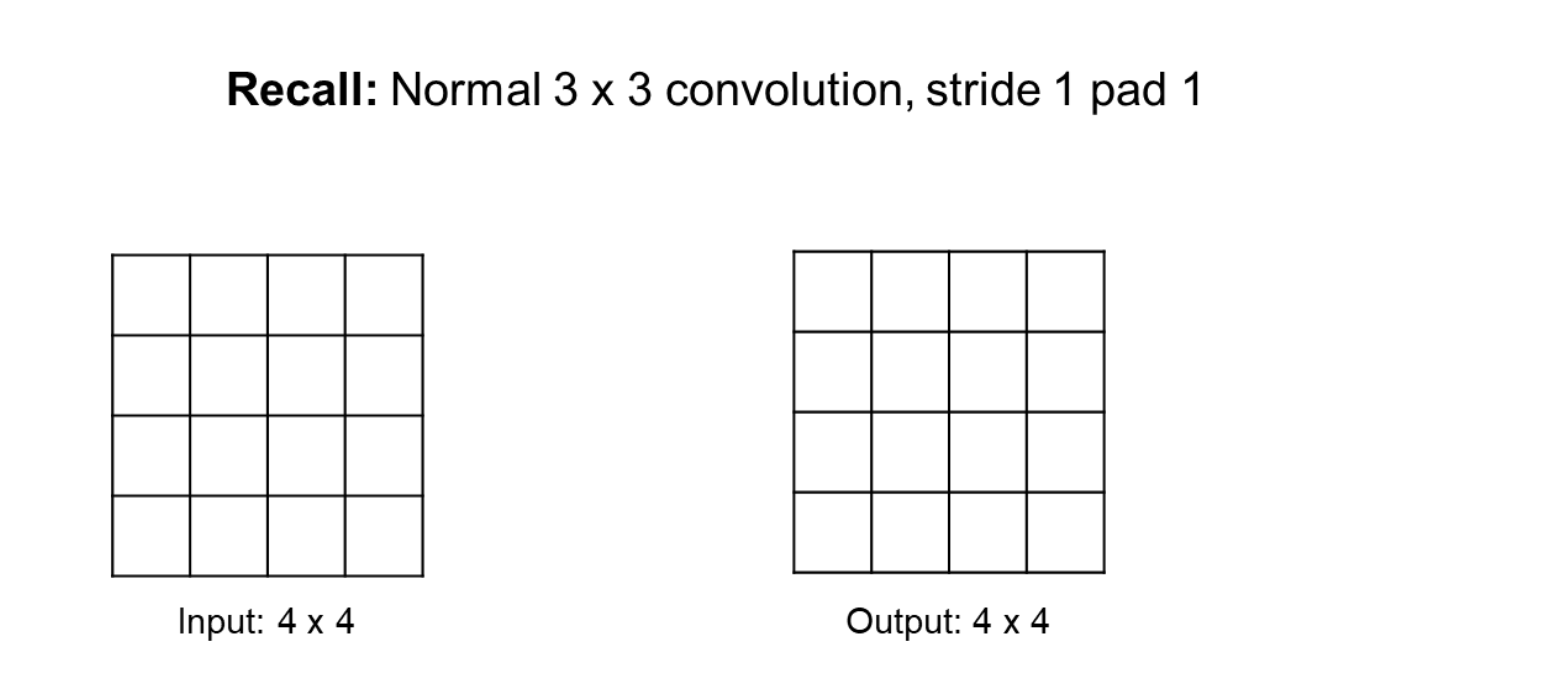
\includegraphics[width=\textwidth]{pic/Transpose conv eg1.png} 
    \end{center}
\end{frame}


\begin{frame}{Learnable Upsampling: “Transpose Convolution”}

    \begin{center}
        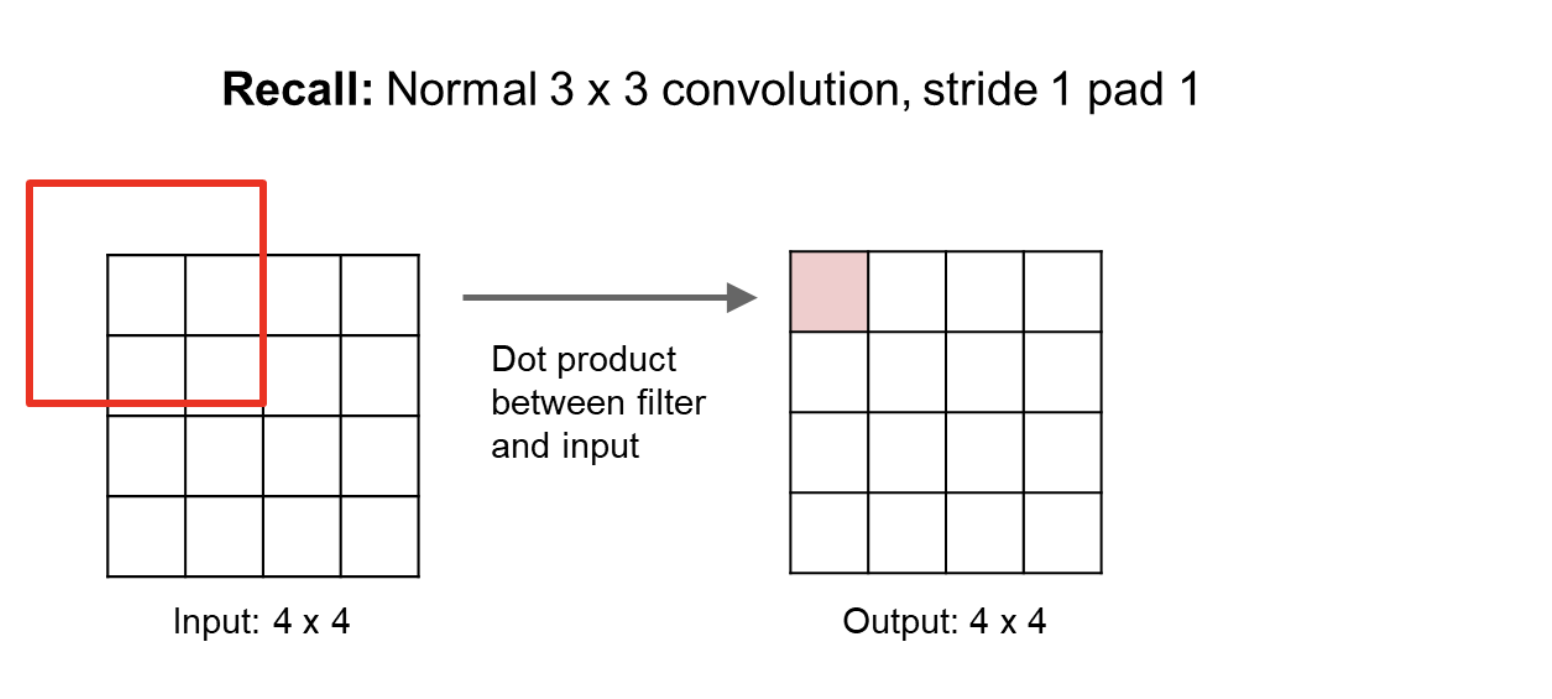
\includegraphics[width=\textwidth]{pic/Transpose conv eg2.png} 
    \end{center}
\end{frame}

\begin{frame}{Learnable Upsampling: “Transpose Convolution”}

    \begin{center}
        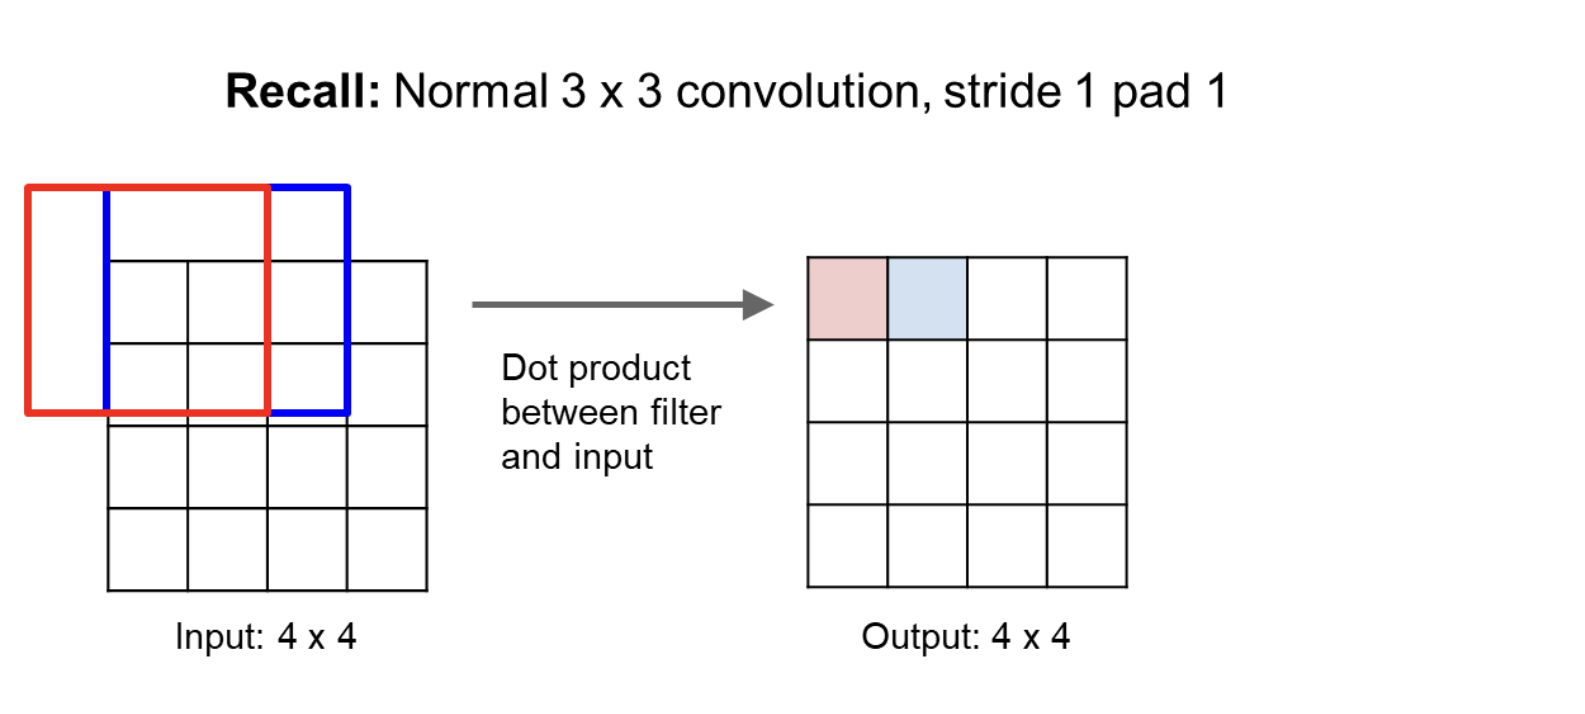
\includegraphics[width=\textwidth]{pic/Transpose conv eg3.png} 
    \end{center}
\end{frame}

\begin{frame}{Learnable Upsampling: “Transpose Convolution”}

    \begin{center}
        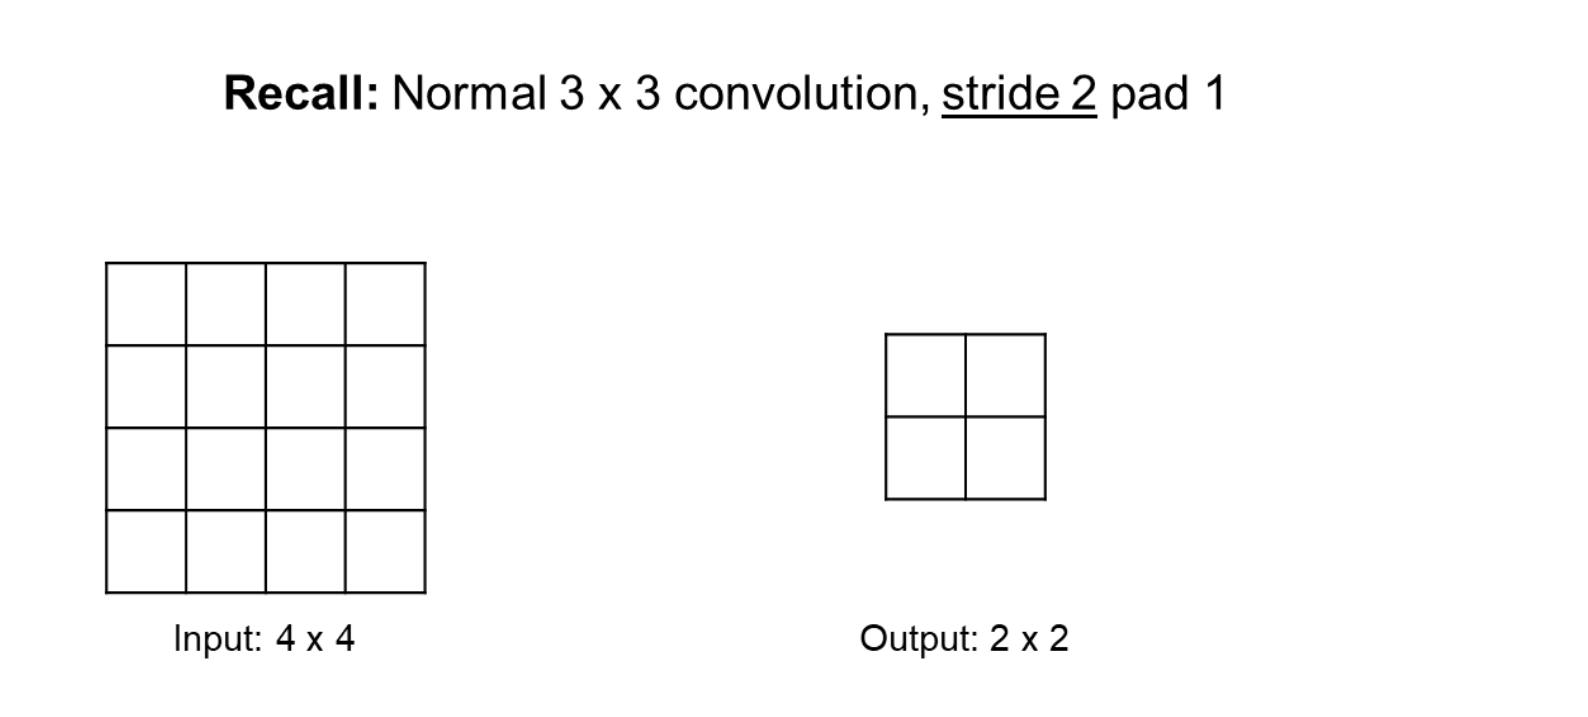
\includegraphics[width=\textwidth]{pic/Transpose conv eg4.png} 
    \end{center}
\end{frame}

\begin{frame}{Learnable Upsampling: “Transpose Convolution”}

    \begin{center}
        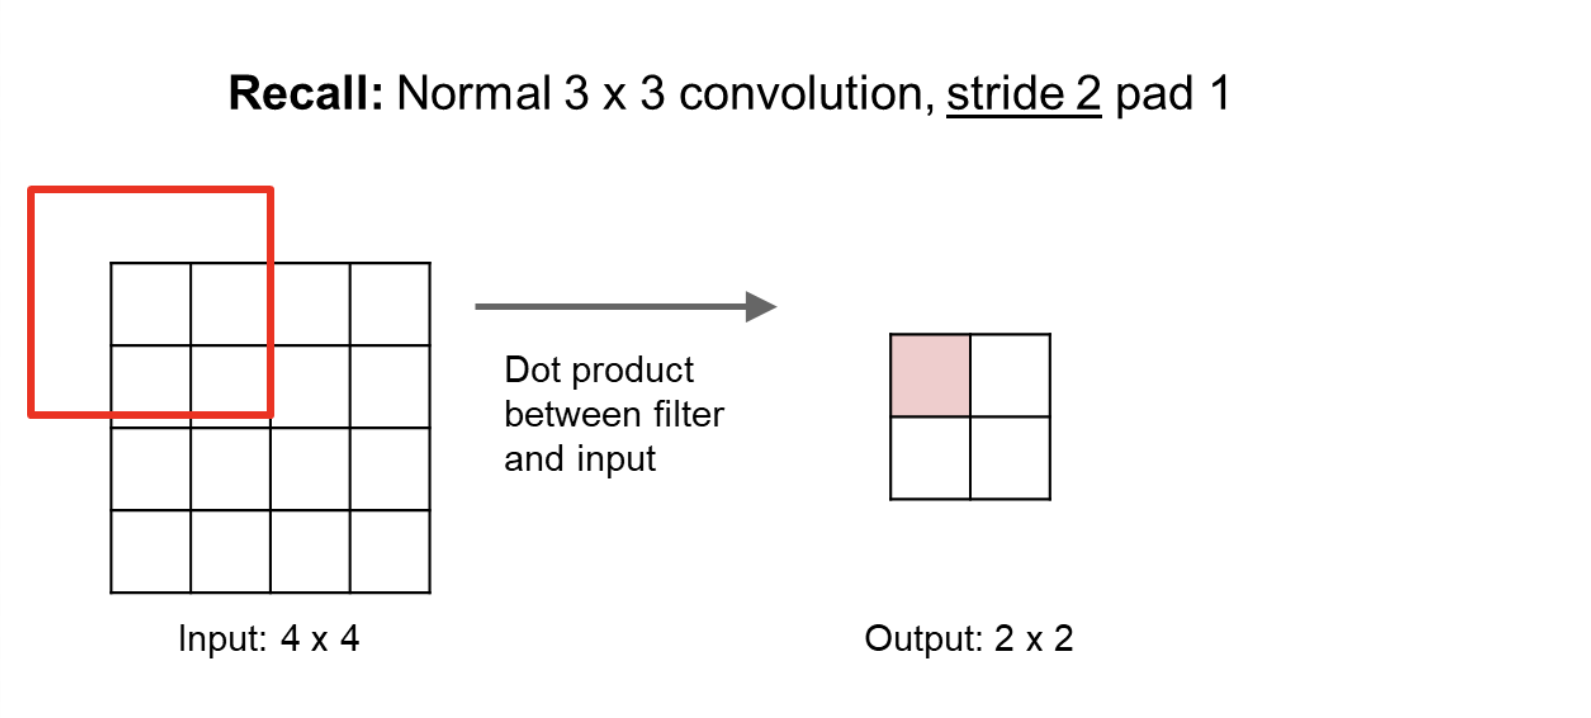
\includegraphics[width=\textwidth]{pic/Transpose conv eg5.png} 
    \end{center}
\end{frame}

\begin{frame}{Learnable Upsampling: “Transpose Convolution”}

    \begin{center}
        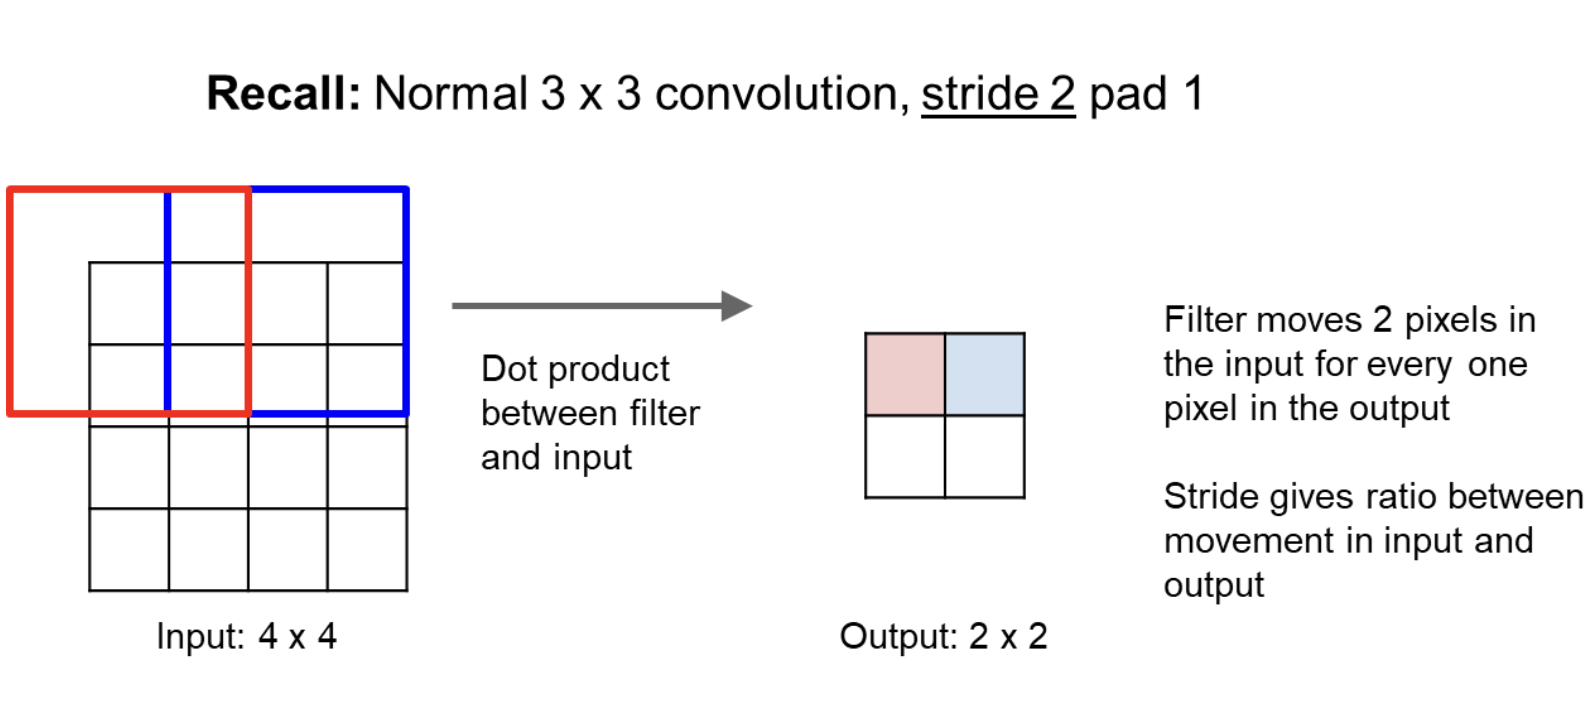
\includegraphics[width=\textwidth]{pic/Transpose conv eg6.png} 
    \end{center}
\end{frame}

\begin{frame}{Learnable Upsampling: “Transpose Convolution”}

    \begin{center}
        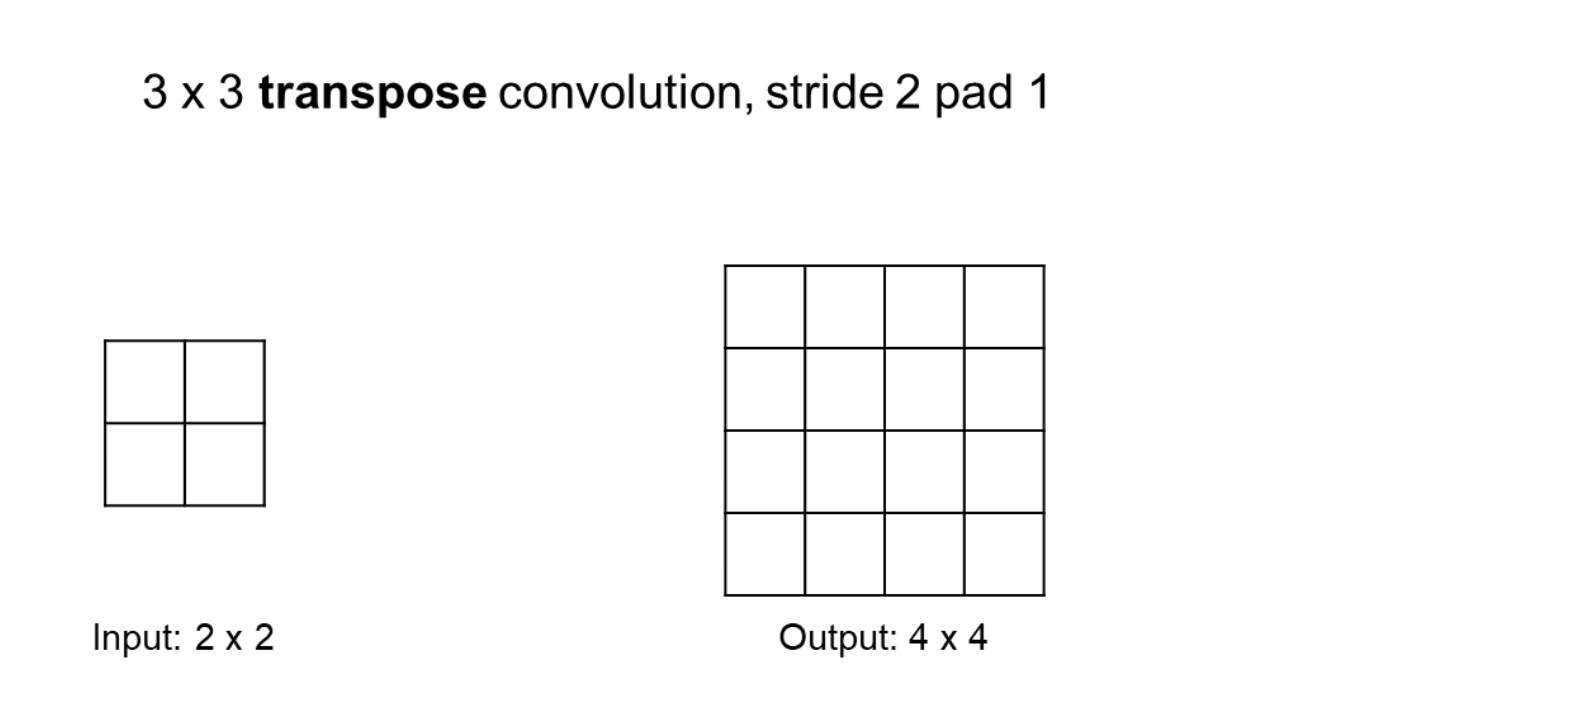
\includegraphics[width=\textwidth]{pic/Transpose conv eg7.png} 
    \end{center}
\end{frame}

\begin{frame}{Learnable Upsampling: “Transpose Convolution”}

    \begin{center}
        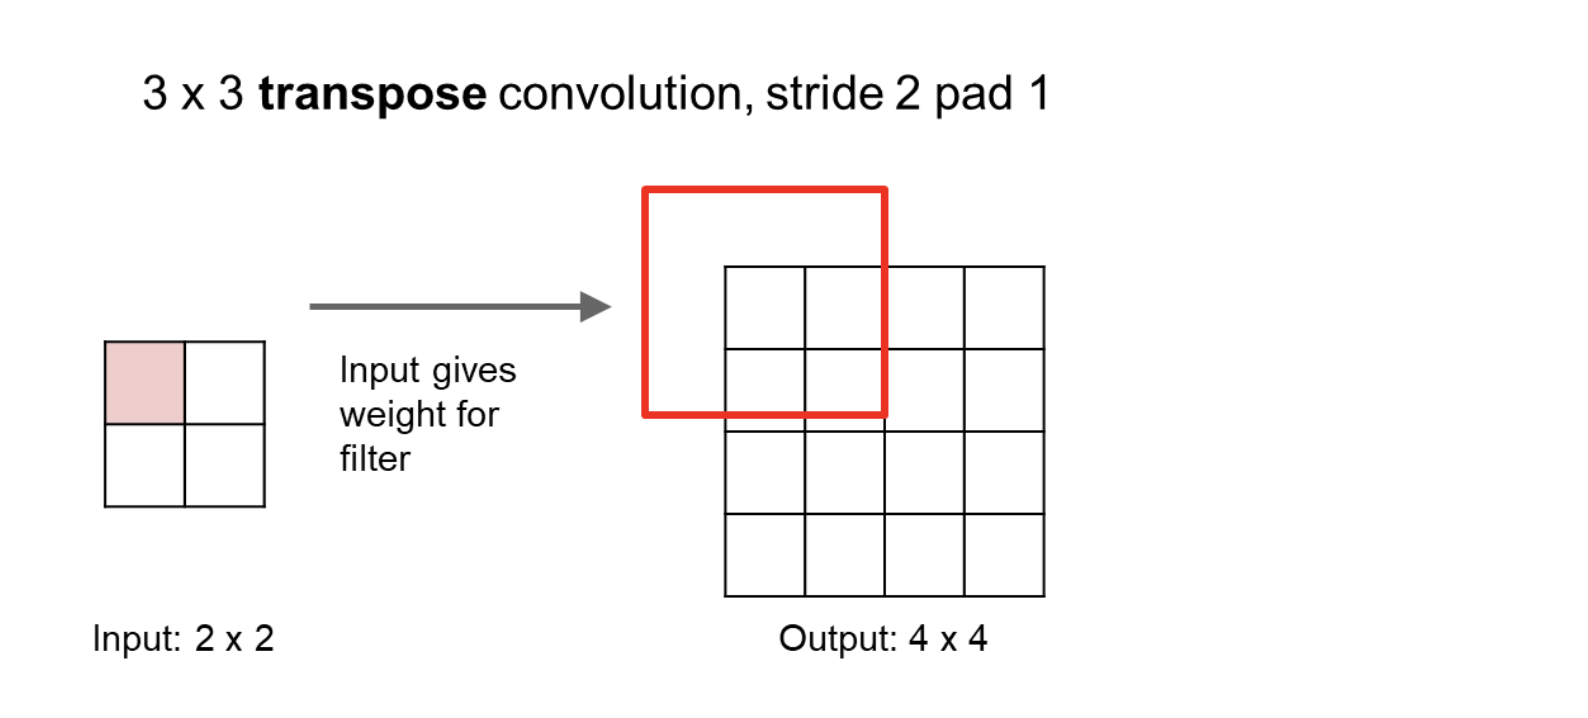
\includegraphics[width=\textwidth]{pic/Transpose conv eg8.png} 
    \end{center}
\end{frame}

\begin{frame}{Learnable Upsampling: “Transpose Convolution”}

    \begin{center}
        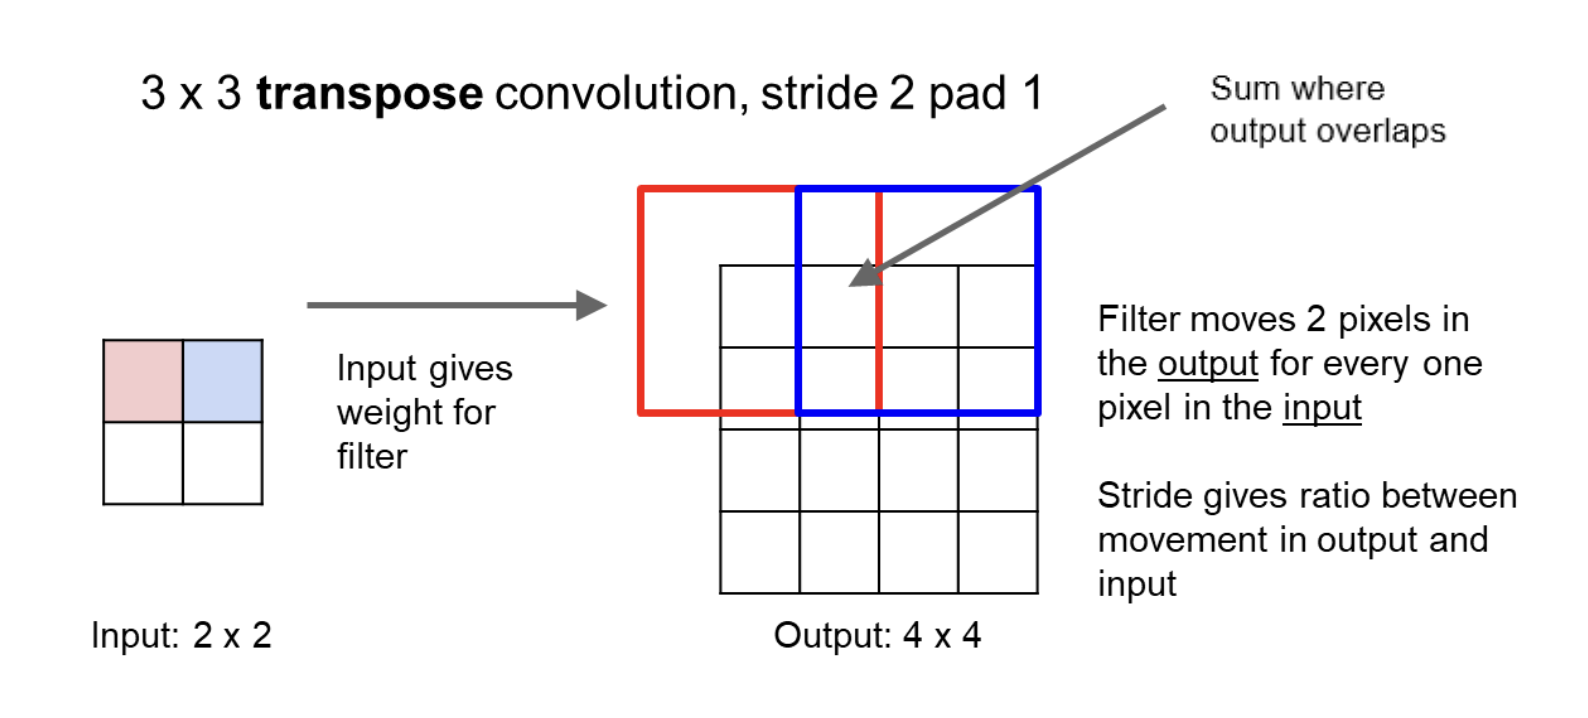
\includegraphics[width=\textwidth]{pic/Transpose conv eg9.png} 
    \end{center}
\end{frame}



\begin{frame}{Transpose Convolution: 1D Example}
    \begin{columns}[T]
        % Left column for Input, Filter, and Output diagram
        \begin{column}{0.75\textwidth}
            \centering
            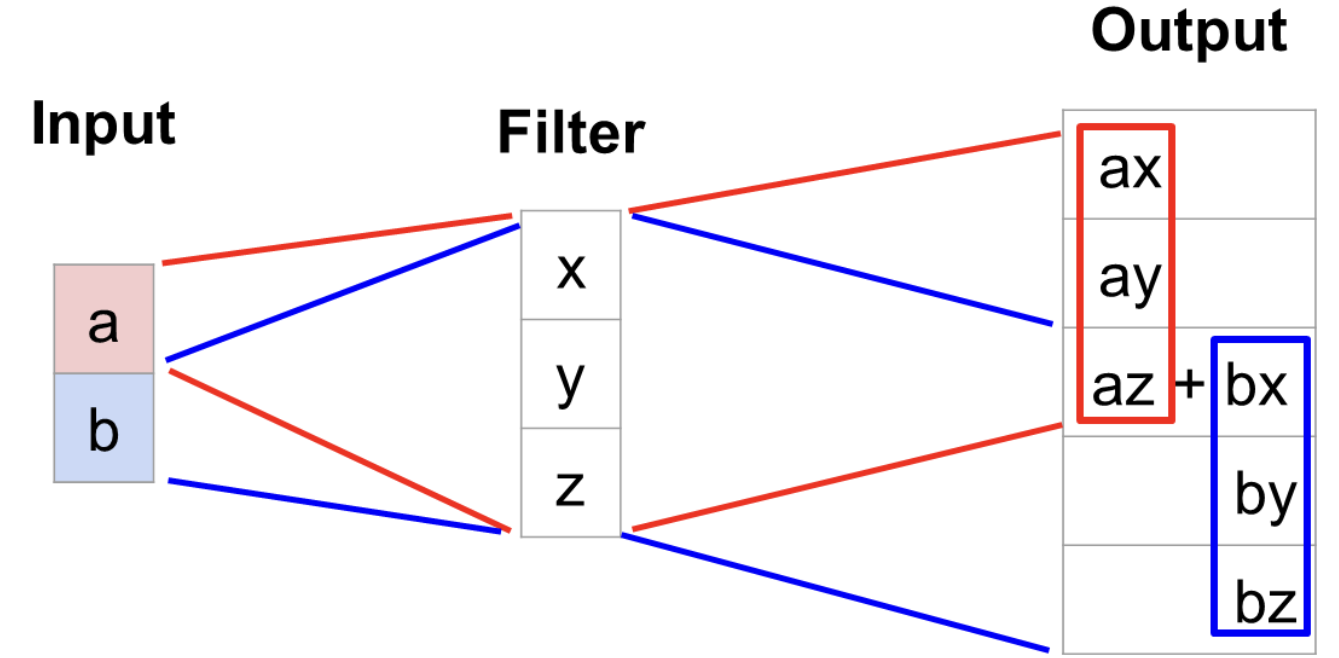
\includegraphics[width=\textwidth]{pic/Transpose Conv 1d example.png}
        \end{column}

        % Right column for explanation text
        \begin{column}{0.35\textwidth}
            \small
            \vspace{1cm}
            \begin{itemize}
                \item \textbf{Output} contains copies of the filter weighted by the \textbf{input}, summing at overlaps in the output.
                \item \textbf{Need to crop} one pixel from the output to make it exactly \textbf{2x input}.
            \end{itemize}
        \end{column}
    \end{columns}
\end{frame}


\begin{frame}{Transpose Convolution: 2D Example}

    \begin{center}
        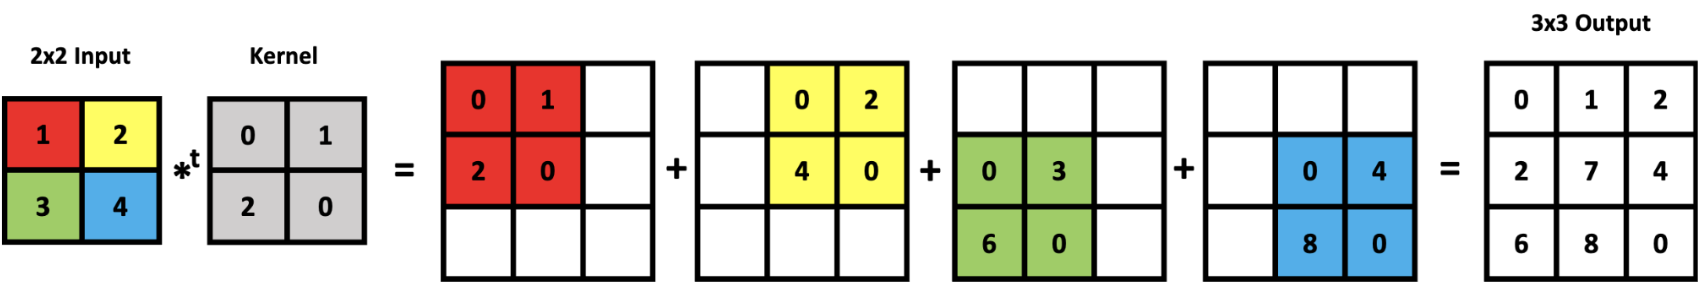
\includegraphics[width=1.05\textwidth]{pic/Transpose Conv 2d example.png} 
    \end{center}

    \vspace{0.6cm}
    \tiny{Image from \href{https://mriquestions.com/upsampling.html}{this link}}
\end{frame}


\section{Case Study: U-Net}


\begin{frame}{U-Net: Purpose \& Origin}
    \begin{itemize}
        \item Developed by Olaf Ronneberger, Philipp Fischer, and Thomas Brox.
        \item First released in 2015, presented at the International Conference on Medical Image Computing and Computer-Assisted Intervention (MICCAI).
        \item Designed specifically for biomedical \textcolor{deepblue}{image segmentation} tasks.
    \end{itemize}
    \begin{center}
        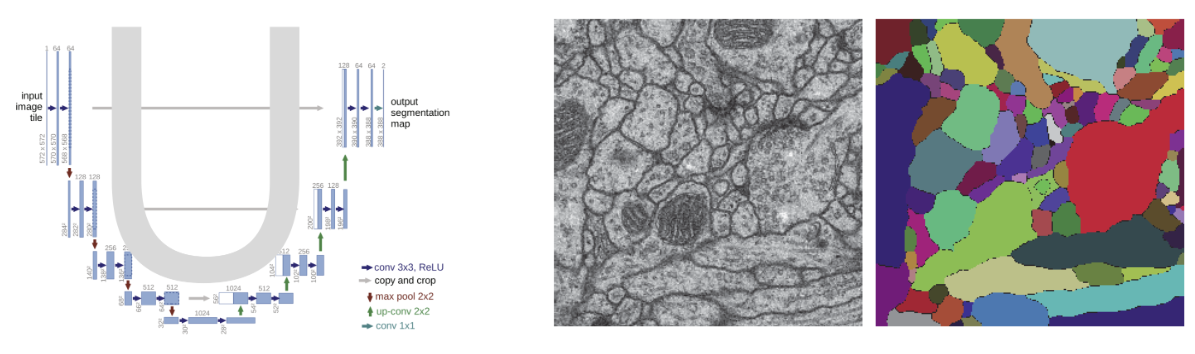
\includegraphics[width=\textwidth]{pic/Unet origin.png} 
    \end{center}

    \vspace{0.3cm}
    \tiny{Image from \href{https://miro.medium.com/v2/resize:fit:1078/1*Dpmg8bywcabPdX08BtlleQ.png}{this link}}
\end{frame}


\begin{frame}{U-Net: Usage Over Time}
    \begin{itemize}
        \item The rise in its usage is due to its simplicity, effectiveness, and adaptability to various image processing tasks beyond medical imaging.
    \end{itemize}

    \begin{center}
        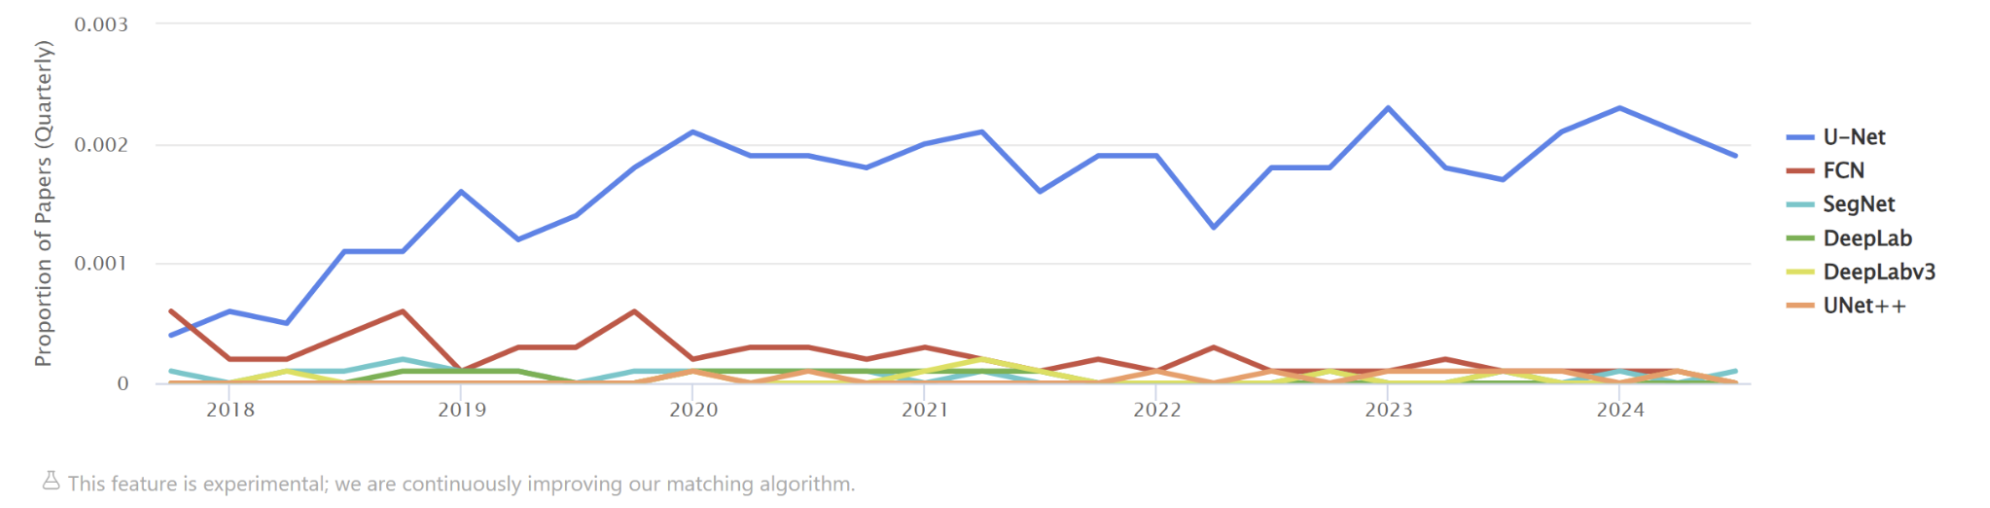
\includegraphics[width=\textwidth]{pic/Unet usage.png} 
    \end{center}

    \vspace{1.4cm}
    \tiny{From \href{https://paperswithcode.com/method/u-net}{papers with code}}
\end{frame}



\begin{frame}{U-Net: Tasks}

    \begin{center}
        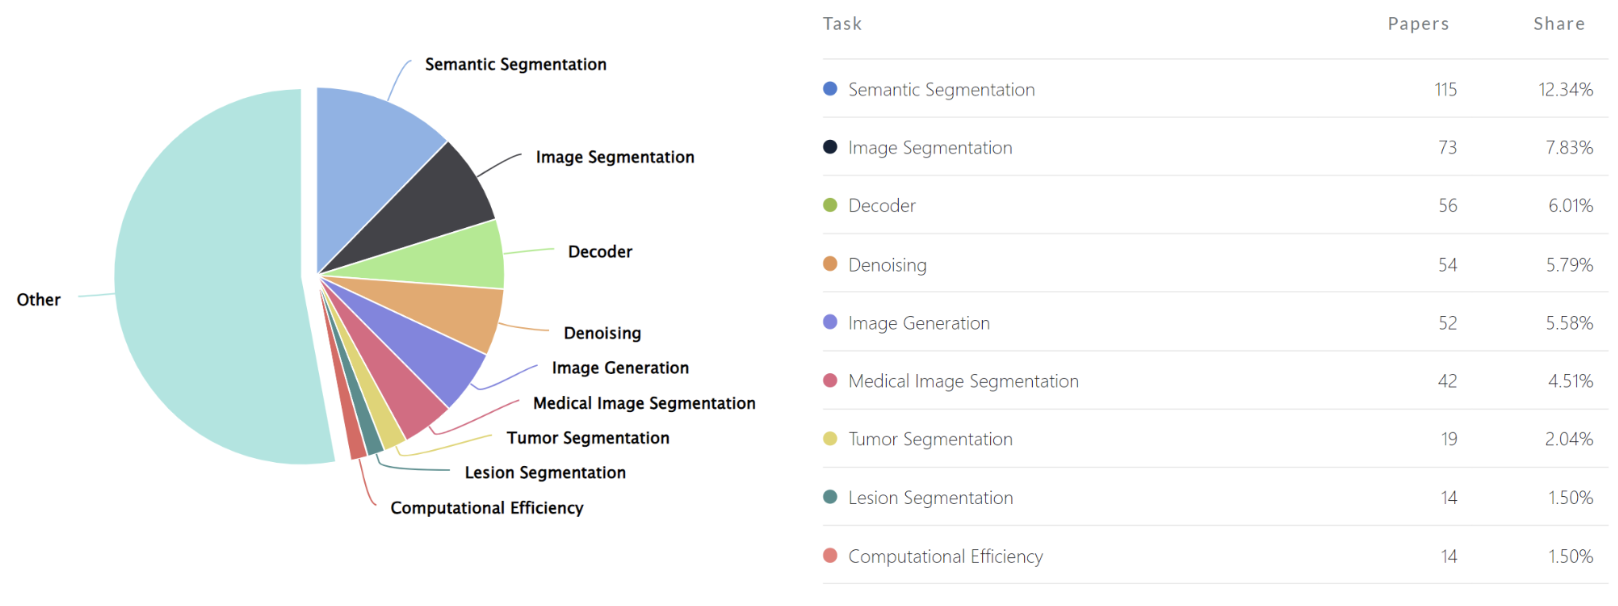
\includegraphics[width=1.05\textwidth]{pic/Unet Tasks.png} 
    \end{center}

    \vspace{0.6cm}
    \tiny{From \href{https://paperswithcode.com/method/u-net}{papers with code}}
\end{frame}


\begin{frame}{U-Net: Big Picture}

    \begin{center}
        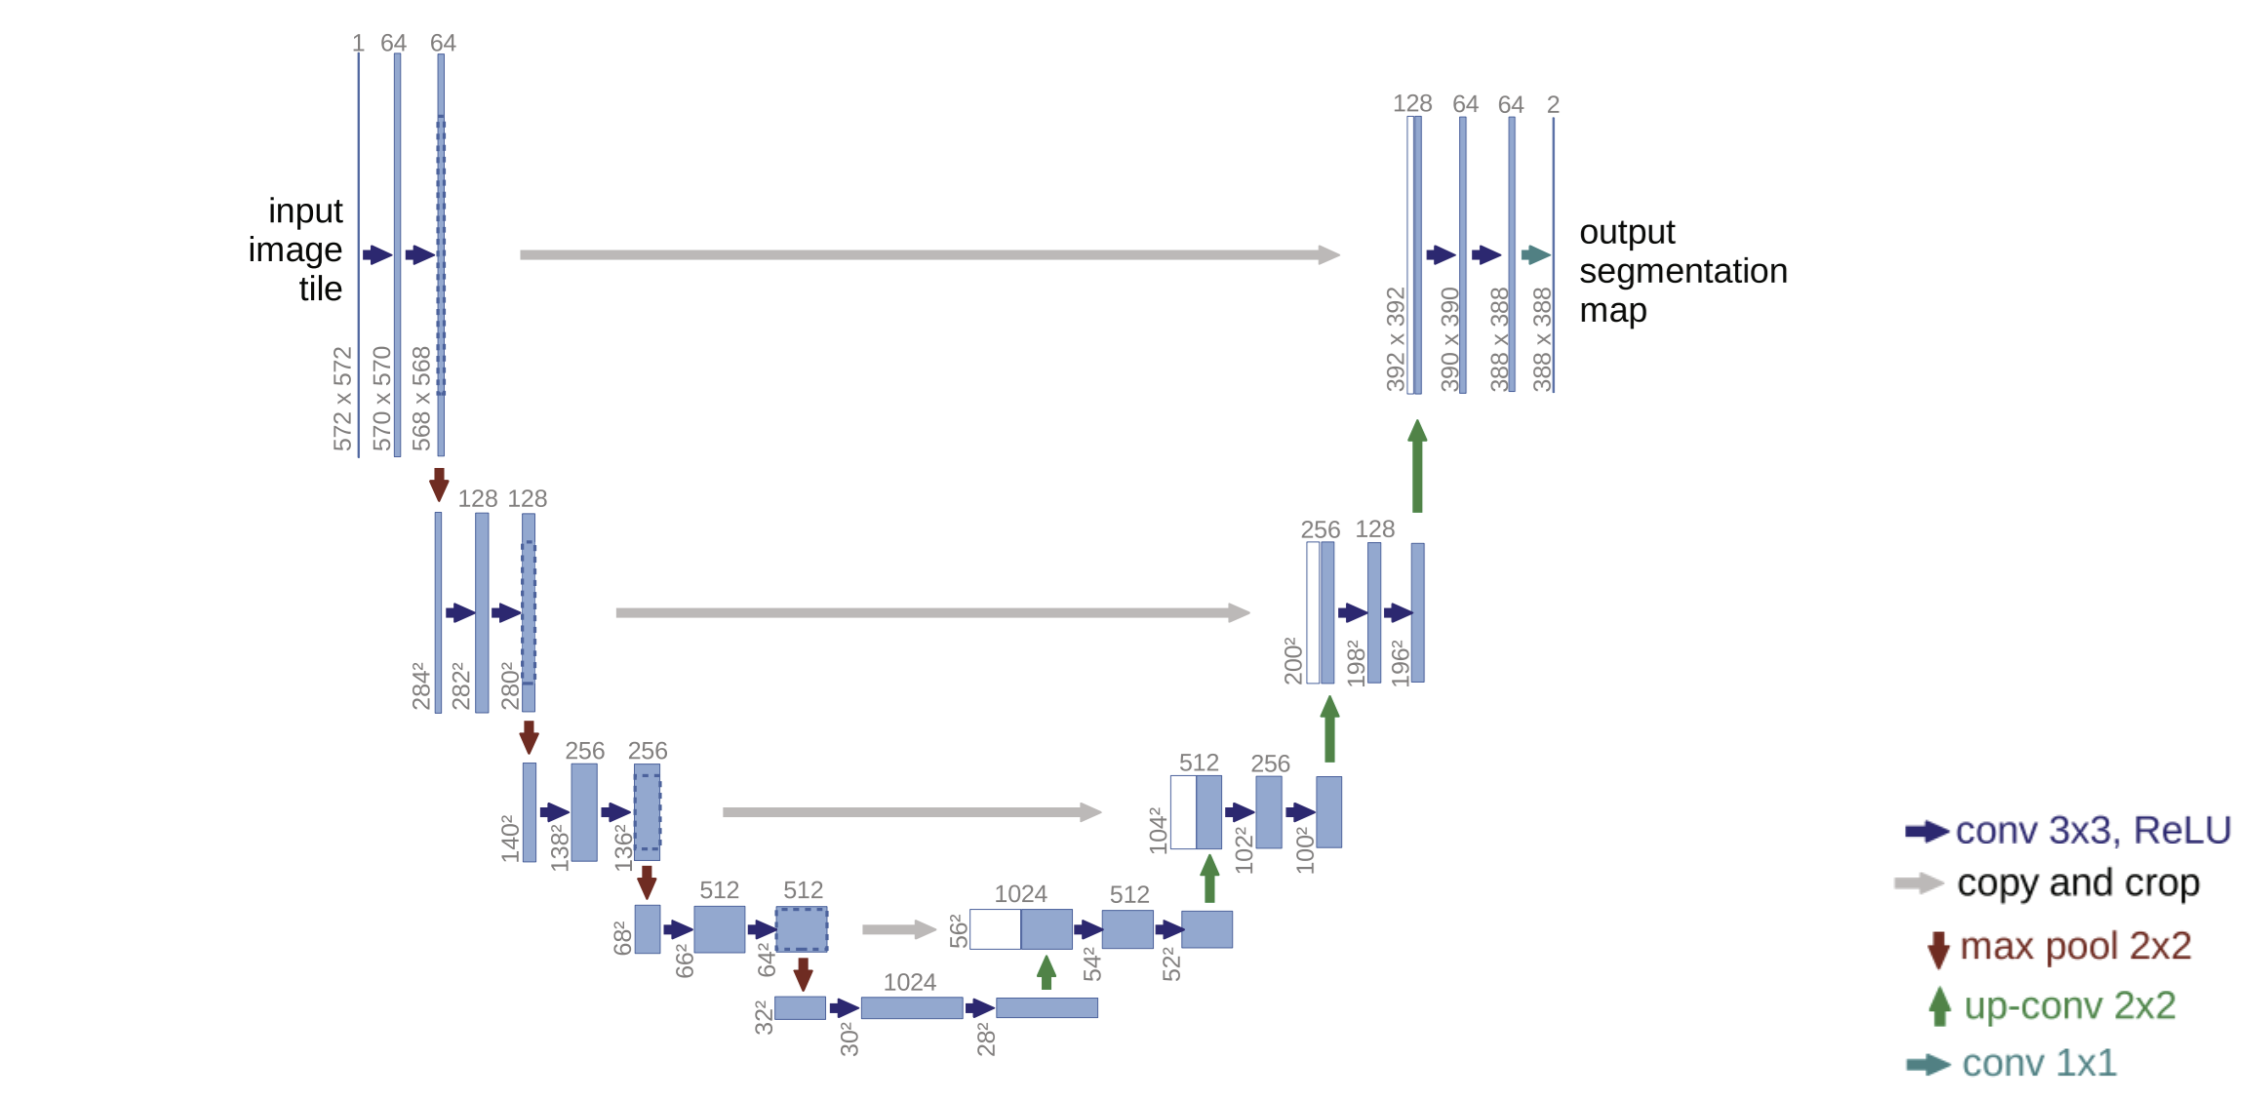
\includegraphics[width=0.95\textwidth]{pic/Unet big pic1.png} 
    \end{center}
    \tiny{From \href{https://arxiv.org/abs/1505.04597}{Unet}}
\end{frame}


\begin{frame}{U-Net: Skip Connections}

    \begin{center}
        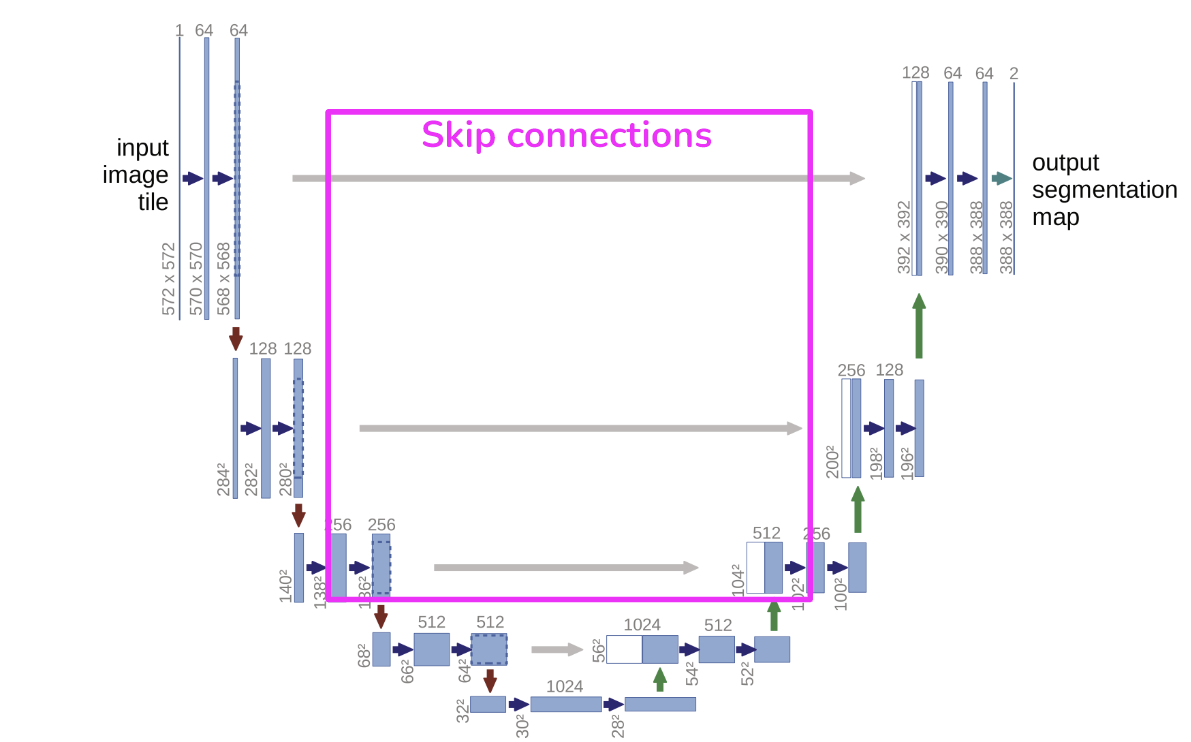
\includegraphics[width=0.75\textwidth]{pic/Unet-Skip connections.png} 
    \end{center}
    \tiny{From \href{https://arxiv.org/abs/1505.04597}{Unet}}
\end{frame}


\begin{frame}{U-Net vs AE's: The Skip Connection's}
\small
\textbf{Preserving Spatial Features \& Reducing Information Bottlenecks:}
\begin{itemize}
    \item Without skip connections, deep layers compress data heavily, leading to loss of spatial details, blurry outputs, and poor segmentation quality, especially in fine edges and boundaries.
    \item Skip connections bypass the bottleneck by passing high-resolution spatial details directly from encoder to decoder, helping retain sharpness and segmentation accuracy.
\end{itemize}

\vspace{0.5cm}

\textbf{Improving Network Stability and Learning:}
\begin{itemize}
    \item Skip connections allow gradients to flow more effectively during backpropagation, mitigating the vanishing gradient problem common in deep networks.
\end{itemize}

\end{frame}



\begin{frame}{U-Net vs AE's: Latent Space}
\small

\textcolor{red}{\textbf{Unlike AE’s (specially VAE), U-Net’s latent space is less expressive:}}

\begin{itemize}
    \item \textbf{Skip Connections Reduce the Bottleneck's Importance:} Because of skip connections, U-Net doesn’t rely solely on the latent space for feature representation. Thus, the latent space is not required to encode as much high-frequency information as in an AE. As a result, its representation isn’t as structured or “clustered,” meaning a t-SNE plot of U-Net’s latent space would not show the same level of clustering we see with VAEs, where every detail must be inferred from the bottleneck.
    
    \vspace{0.3cm}
    
    \item \textbf{No Strong Encoding Constraint:} Since skip connections provide spatial detail, U-Net’s latent space is not forced to develop an “expressive” representation, which is essential for models like VAEs where information passes strictly through a bottleneck.
\end{itemize}

\end{frame}



\begin{frame}{U-Net: Big Picture}

    \begin{center}
        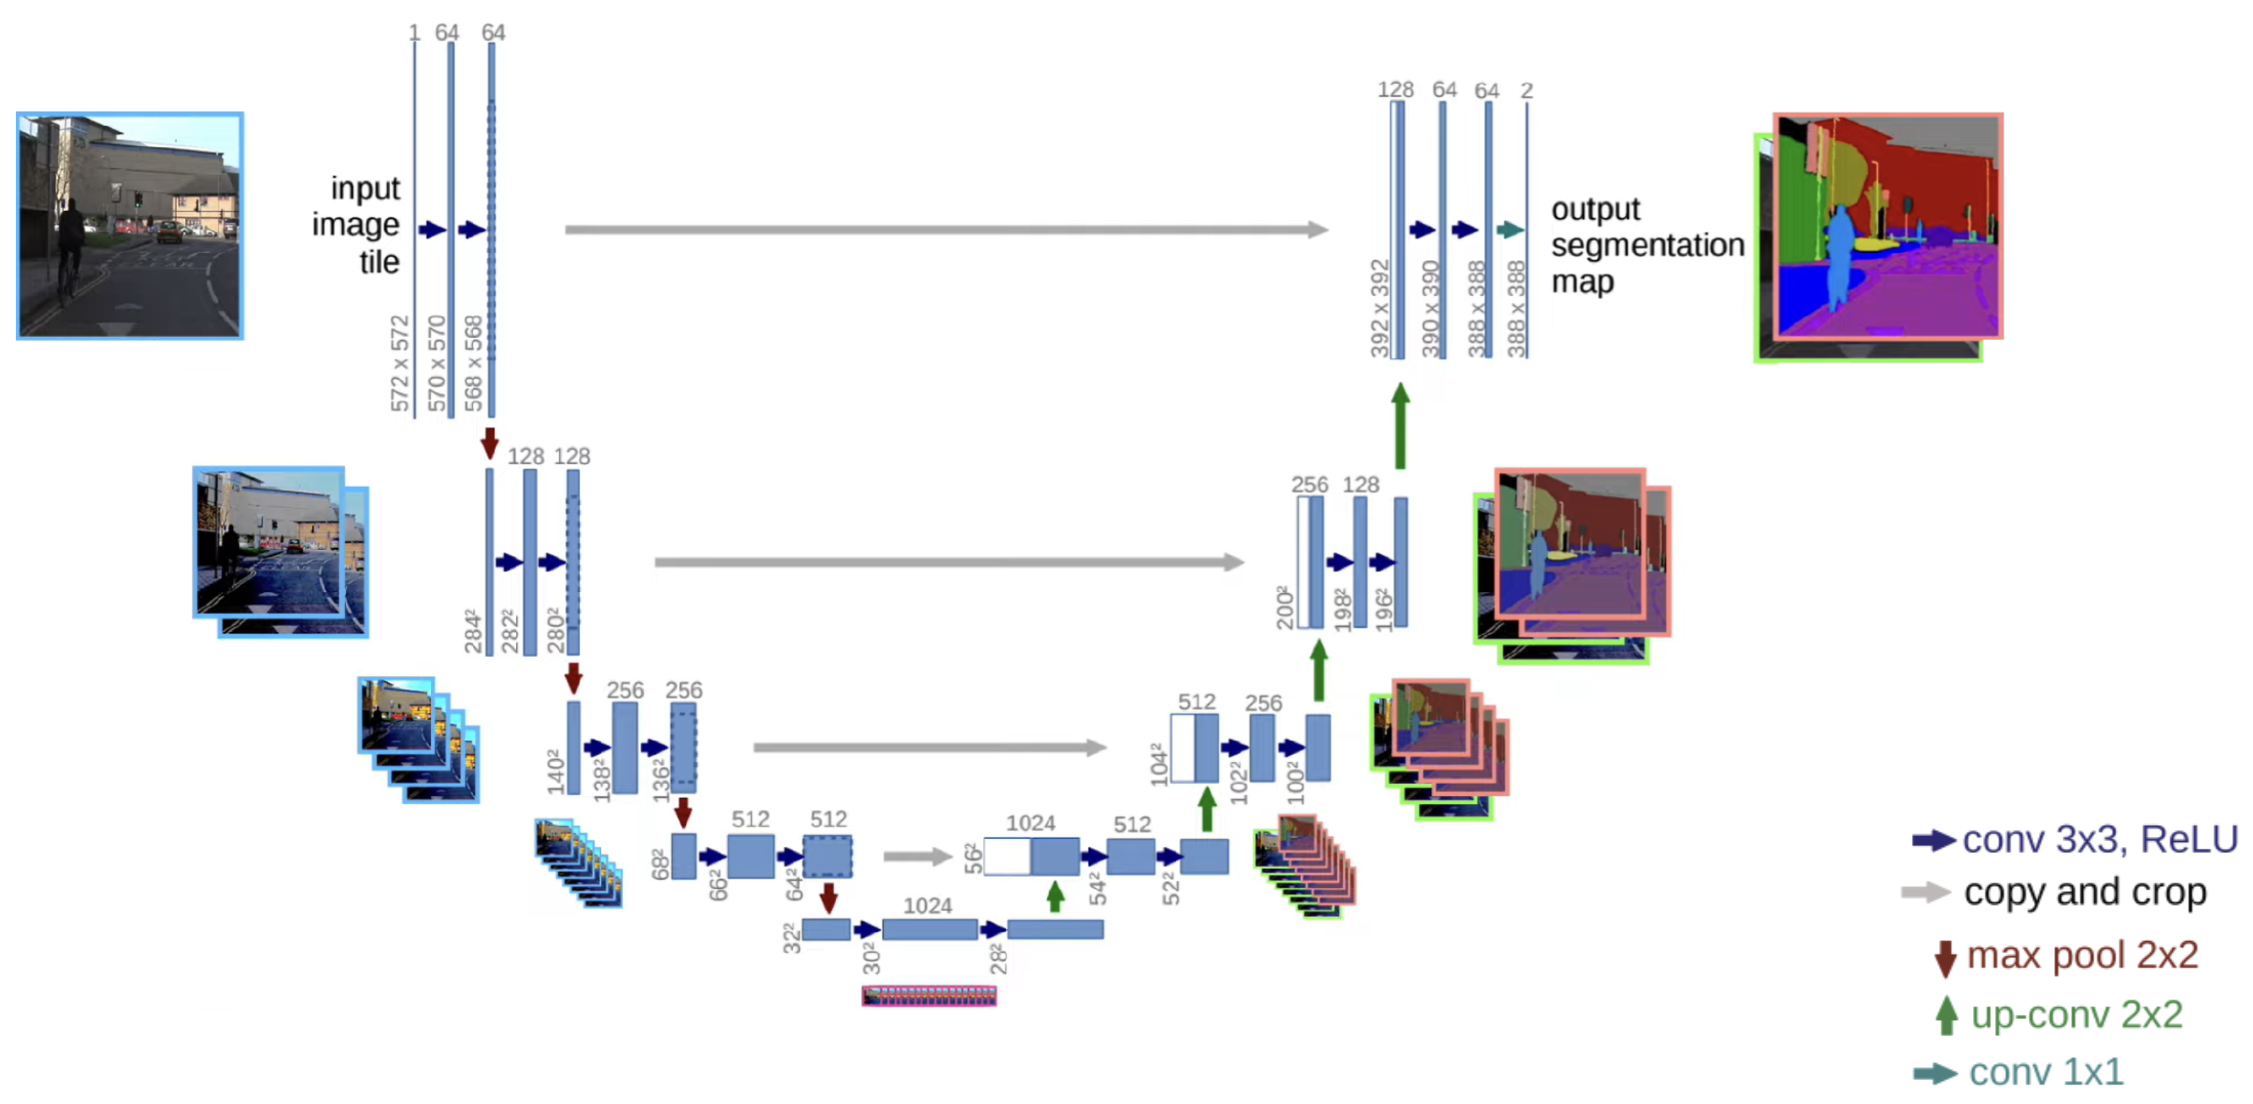
\includegraphics[width=0.95\textwidth]{pic/Unet big picture3.png} 
    \end{center}
    \tiny{From \href{https://www.youtube.com/watch?v=NhdzGfB1q74}{this link}}
\end{frame}



\begin{frame}{U-Net: Big Picture}

    \begin{center}
        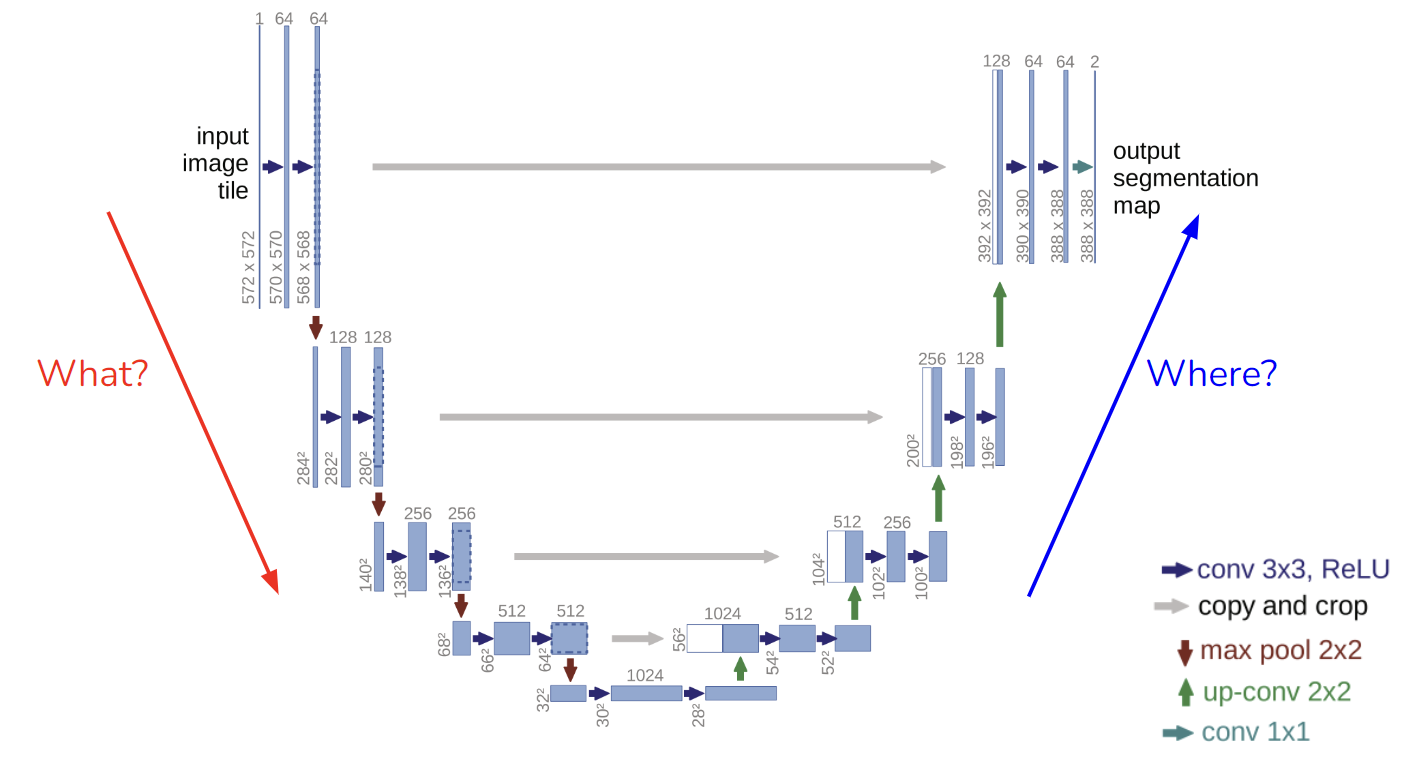
\includegraphics[width=0.85\textwidth]{pic/Unet big picture4.png} 
    \end{center}
    \tiny{From \href{https://arxiv.org/abs/1505.04597}{Unet}}
\end{frame}



\begin{frame}{U-Net: Big Picture}

    \begin{center}
        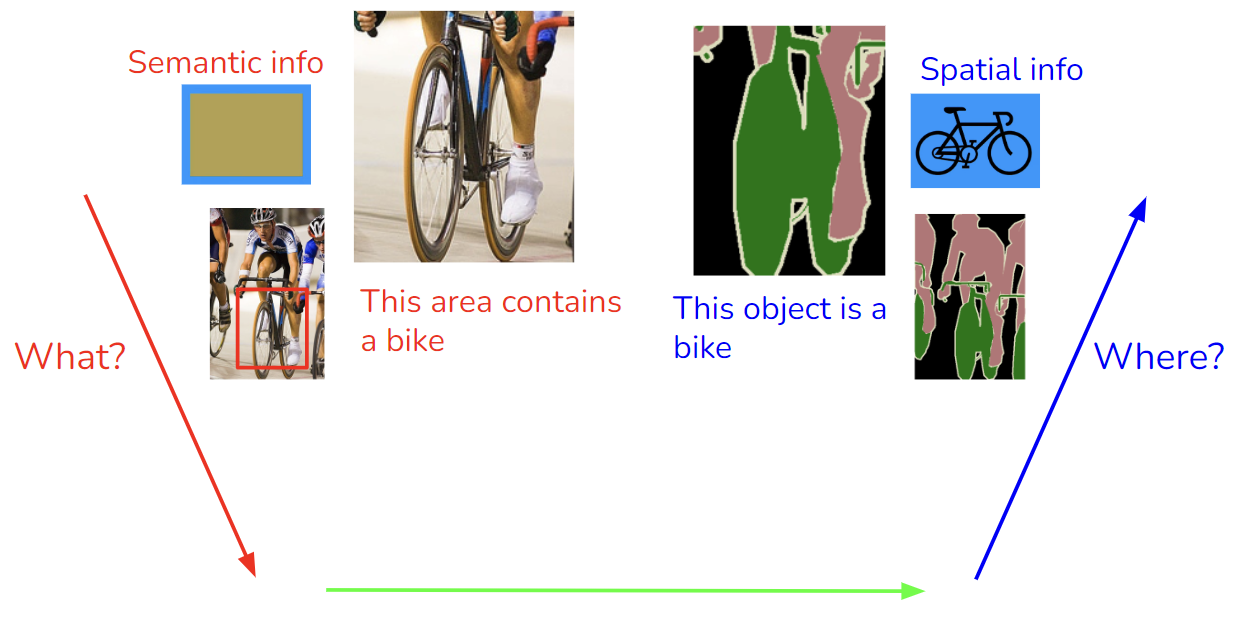
\includegraphics[width=0.95\textwidth]{pic/Unet big picture5.png} 
    \end{center}
    \tiny{From \href{https://www.youtube.com/watch?v=NhdzGfB1q74}{this link}}
\end{frame}



\begin{frame}{U-Net: Encoder}

    \begin{center}
        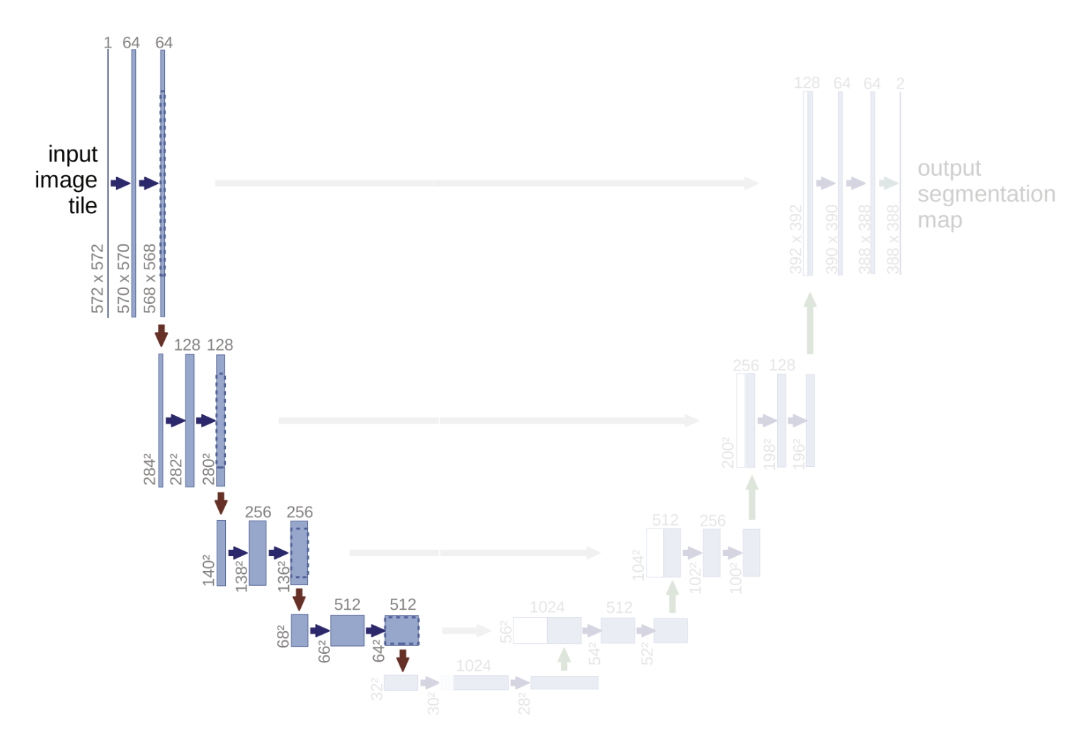
\includegraphics[width=0.7\textwidth]{pic/Unet-Encoder1.png} 
    \end{center}
\end{frame}

\begin{frame}{U-Net: Encoder}
    \begin{columns}[T] % Split the frame into two vertical columns
    
        % Left Column
        \begin{column}{0.7\textwidth}
            \begin{itemize}
            \scriptsize
                \item Repeated 3x3 convolutional with \textbf{\textcolor{red!60!black}{valid padding}} (= no padding) + ReLU layers
                \item 2x2 max pooling layers to down sample
                \item \textbf{\textcolor{yellow!60!black}{Double channels}} with conv after the \textbf{\textcolor{green!60!black}{max pool}}
                \item Due to the \textbf{\textcolor{blue!60!black}{shrinking effect}} of valid convs, \textbf{\textcolor{cyan!60!black}{cropped part}} is concatenated with upsampled feature map
            \end{itemize}
            % Shift figure slightly to the right
            \begin{center}
                \hspace{0.5cm} % Adjust horizontal spacing
                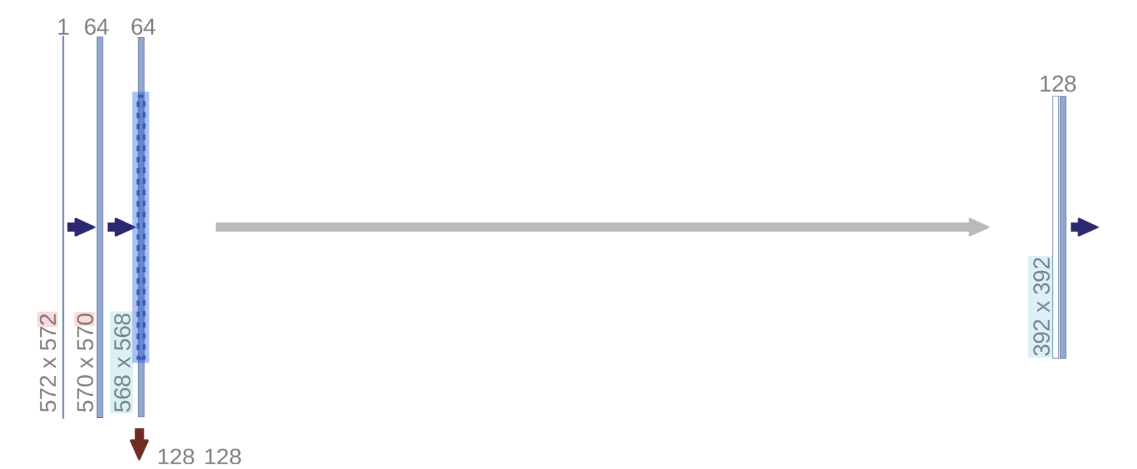
\includegraphics[width=0.9\textwidth]{pic/Unet-Encoder2.png}
            \end{center}
        \end{column}
        
        % Right Column
        \begin{column}{0.2\textwidth}
            % Place Figure 3
            \begin{center}
                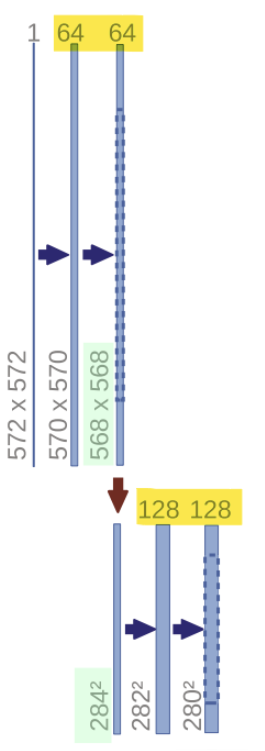
\includegraphics[width=0.7\textwidth]{pic/Unet-Encoder3.png}
                \vspace{3cm}
            \end{center}
        \end{column}
        
    \end{columns}
\end{frame}


\begin{frame}{U-Net: Bottleneck}
    \begin{itemize}
    \small
    \setlength\itemsep{1em} 
        \item Down sample with \textbf{2x2 max pooling}
        \item Repeated \textbf{3x3 convolutional} with \textcolor{red!60!black}{valid pooling} (= no padding) + ReLU layers
        \item \textbf{Double channels} with conv after the max pool
    \end{itemize}

    \begin{center}
        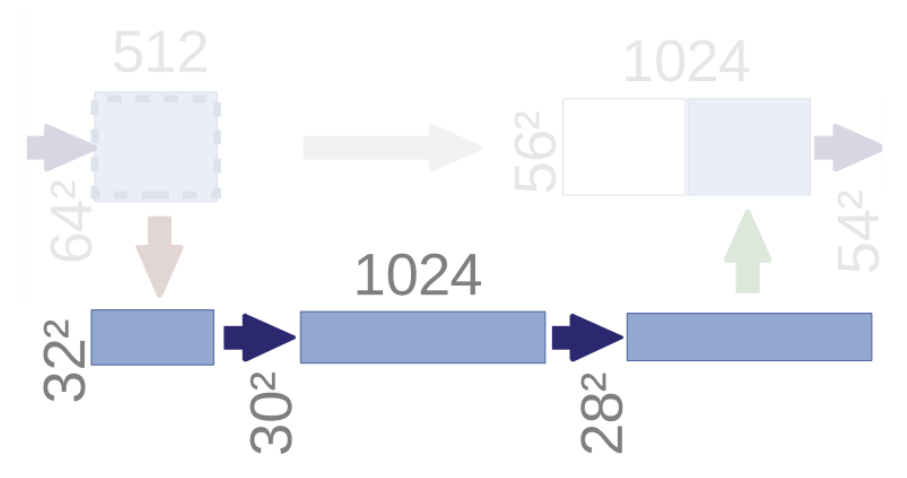
\includegraphics[width=0.5\textwidth]{pic/Unet Bottleneck.png}
    \end{center}
\end{frame}


\begin{frame}{U-Net: Decoder}
    \scriptsize
    \begin{columns} % Use two-column layout
        \begin{column}{0.7\textwidth}
        \vspace{-1cm}
            \begin{itemize}
                \setlength\itemsep{1em} % Adjust spacing between bullet points
                \item Repeated 3x3 convolutional with \textbf{valid pooling} (= no padding) + ReLU layers
                \item Upsampling, followed by 2x2 convolutional layer
                \item Halve channels after upsampling convolution
            \end{itemize}
            
        \end{column}

        % Right column for the figure
        \begin{column}{0.5\textwidth}
            \begin{center}
                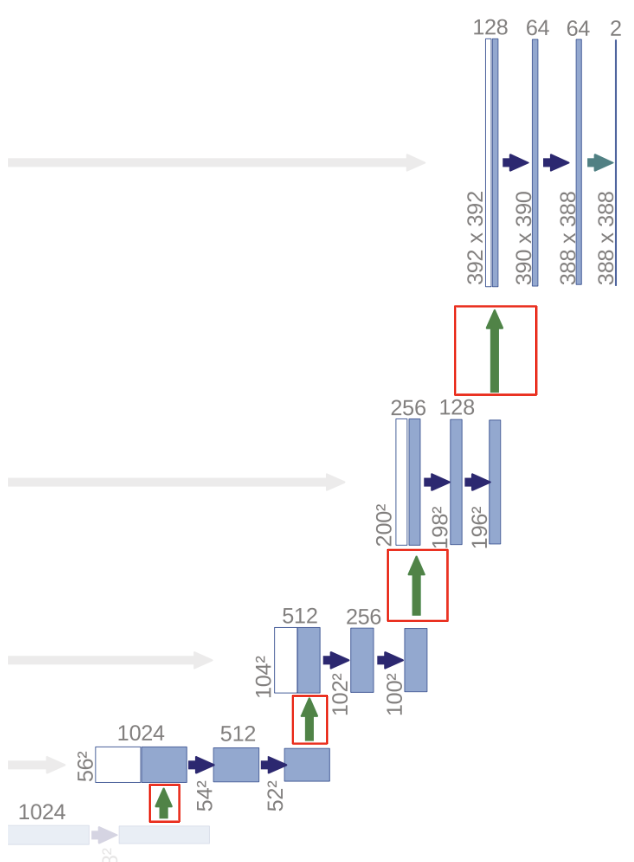
\includegraphics[width=0.6\textwidth]{pic/Unet decoder.png} 
            \end{center}
        \end{column}
    \end{columns}
\end{frame}



\begin{frame}{U-Net: Skip Connections}
\small
    \textbf{Skip Connections:}
    \begin{itemize}
        \item Connect encoder layers to decoder layers at the same depth.
        \item Preserve high-resolution features for better upsampling.
    \end{itemize}
    
    \vspace{0.5cm} % Add vertical space between sections
    
    \textbf{Cropping for Alignment:}
    \begin{itemize}
        \item Due to valid padding, feature maps in the encoder are larger than those in the decoder.
        \item Cropping aligns sizes before concatenation in skip connections.
    \end{itemize}
    
    \vspace{0.5cm} % Add vertical space between sections
    
    \textbf{Why Important?:}
    \begin{itemize}
        \item Combines local details (from encoder) with context (from decoder).
        \item Helps in precise pixel-wise segmentation.
        \item Overcomes vanishing gradient issue by allowing smooth information flow.
    \end{itemize}
\end{frame}





\begin{frame}{Data Efficiency in U-Net}
\scriptsize
\begin{itemize}
    \item \textbf{Residual and Skip Connections:} These connections reduce the amount of information the model needs to learn, as many spatial details are preserved, requiring less adaptation from the model. The need to learn detailed spatial arrangements is mitigated by direct concatenation, which efficiently reintroduces spatial information.
    \vspace{0.3cm}
    \item \textbf{Fully Convolutional Nature:} U-Net uses only convolutional layers, which have fewer parameters compared to fully connected networks. This allows the model to generalize well from smaller datasets.
    \vspace{0.3cm}
    \item \textbf{Data Augmentation Advantages:} Because U-Net is often used for pixel-wise tasks like semantic segmentation, every augmentation (rotation, scaling, etc.) maintains a one-to-one correspondence with ground truth masks. This allows each augmentation to act as a ``new'' data point, further enriching the dataset without additional manual labeling.
    \vspace{0.3cm}
    \item \textbf{Patch-Based Training:} Instead of processing the entire image (e.g., a 1024x1024 image), U-Net can work with smaller patches, increasing batch sizes and enabling more efficient use of each image during training.
\end{itemize}
\end{frame}




\section{References}

\begin{frame}[allowframebreaks]
    \bibliography{ref}
    \bibliographystyle{ieeetr}
    \nocite{*} % used here because no citation happens in slides
    \small
    \textbf{Slides by: Amirhossein Izadi}
    \begin{itemize}
        \item F.-F. Li, J. Wu, and R. Gao, “CS231n” Lecture slides, 2024, Stanford 
        \item A. Amini, “6s191” Lecture slides, 2024, MIT. 
        \item M. Soleymani, “Deep Learning” Lecture slides, 2024, Sharif University of Technology.
        \item H. Beigy, “Deep Learning” Lecture slides, 2022, Sharif University of Technology.
        \item S. Levine, “CS W182/282A” Lecture slides, 2024, UC Berkeley 
        \item Y. Maziane, “Diffusion models: Seek of information and structure in latent space,” 2022, University of Liège.
        \item G. Buzzard, “Mathematical Aspects of Neural Networks” Lecture slides, 2019, Purdue University.
    \end{itemize}
\end{frame}


\begin{frame}
    \begin{center}
        {\Huge Any Questions?}
    \end{center}
\end{frame}

\end{document}